%!TEX TS-program = xelatex
\documentclass[11pt]{article}

\usepackage[english]{babel}

\usepackage{amsmath,amssymb,amsfonts}
\usepackage[utf8]{inputenc}
\usepackage[T1]{fontenc}
\usepackage{stix2}
\usepackage[scaled]{helvet}
\usepackage[scaled]{inconsolata}

\usepackage{lastpage}

\usepackage{setspace}

\usepackage{ccicons}

\usepackage[hang,flushmargin]{footmisc}

\usepackage{geometry}

\setlength{\parindent}{0pt}
\setlength{\parskip}{6pt plus 2pt minus 1pt}

\usepackage{fancyhdr}
\renewcommand{\headrulewidth}{0pt}\providecommand{\tightlist}{%
  \setlength{\itemsep}{0pt}\setlength{\parskip}{0pt}}

\makeatletter
\newcounter{tableno}
\newenvironment{tablenos:no-prefix-table-caption}{
  \caption@ifcompatibility{}{
    \let\oldthetable\thetable
    \let\oldtheHtable\theHtable
    \renewcommand{\thetable}{tableno:\thetableno}
    \renewcommand{\theHtable}{tableno:\thetableno}
    \stepcounter{tableno}
    \captionsetup{labelformat=empty}
  }
}{
  \caption@ifcompatibility{}{
    \captionsetup{labelformat=default}
    \let\thetable\oldthetable
    \let\theHtable\oldtheHtable
    \addtocounter{table}{-1}
  }
}
\makeatother

\usepackage{array}
\newcommand{\PreserveBackslash}[1]{\let\temp=\\#1\let\\=\temp}
\let\PBS=\PreserveBackslash

\usepackage[breaklinks=true]{hyperref}
\hypersetup{colorlinks,%
citecolor=blue,%
filecolor=blue,%
linkcolor=blue,%
urlcolor=blue}
\usepackage{url}

\usepackage{caption}
\setcounter{secnumdepth}{0}
\usepackage{cleveref}

\usepackage{graphicx}
\makeatletter
\def\maxwidth{\ifdim\Gin@nat@width>\linewidth\linewidth
\else\Gin@nat@width\fi}
\makeatother
\let\Oldincludegraphics\includegraphics
\renewcommand{\includegraphics}[1]{\Oldincludegraphics[width=\maxwidth]{#1}}

\usepackage{longtable}
\usepackage{booktabs}

\usepackage{color}
\usepackage{fancyvrb}
\newcommand{\VerbBar}{|}
\newcommand{\VERB}{\Verb[commandchars=\\\{\}]}
\DefineVerbatimEnvironment{Highlighting}{Verbatim}{commandchars=\\\{\}}
% Add ',fontsize=\small' for more characters per line
\usepackage{framed}
\definecolor{shadecolor}{RGB}{248,248,248}
\newenvironment{Shaded}{\begin{snugshade}}{\end{snugshade}}
\newcommand{\KeywordTok}[1]{\textcolor[rgb]{0.13,0.29,0.53}{\textbf{#1}}}
\newcommand{\DataTypeTok}[1]{\textcolor[rgb]{0.13,0.29,0.53}{#1}}
\newcommand{\DecValTok}[1]{\textcolor[rgb]{0.00,0.00,0.81}{#1}}
\newcommand{\BaseNTok}[1]{\textcolor[rgb]{0.00,0.00,0.81}{#1}}
\newcommand{\FloatTok}[1]{\textcolor[rgb]{0.00,0.00,0.81}{#1}}
\newcommand{\ConstantTok}[1]{\textcolor[rgb]{0.00,0.00,0.00}{#1}}
\newcommand{\CharTok}[1]{\textcolor[rgb]{0.31,0.60,0.02}{#1}}
\newcommand{\SpecialCharTok}[1]{\textcolor[rgb]{0.00,0.00,0.00}{#1}}
\newcommand{\StringTok}[1]{\textcolor[rgb]{0.31,0.60,0.02}{#1}}
\newcommand{\VerbatimStringTok}[1]{\textcolor[rgb]{0.31,0.60,0.02}{#1}}
\newcommand{\SpecialStringTok}[1]{\textcolor[rgb]{0.31,0.60,0.02}{#1}}
\newcommand{\ImportTok}[1]{#1}
\newcommand{\CommentTok}[1]{\textcolor[rgb]{0.56,0.35,0.01}{\textit{#1}}}
\newcommand{\DocumentationTok}[1]{\textcolor[rgb]{0.56,0.35,0.01}{\textbf{\textit{#1}}}}
\newcommand{\AnnotationTok}[1]{\textcolor[rgb]{0.56,0.35,0.01}{\textbf{\textit{#1}}}}
\newcommand{\CommentVarTok}[1]{\textcolor[rgb]{0.56,0.35,0.01}{\textbf{\textit{#1}}}}
\newcommand{\OtherTok}[1]{\textcolor[rgb]{0.56,0.35,0.01}{#1}}
\newcommand{\FunctionTok}[1]{\textcolor[rgb]{0.00,0.00,0.00}{#1}}
\newcommand{\VariableTok}[1]{\textcolor[rgb]{0.00,0.00,0.00}{#1}}
\newcommand{\ControlFlowTok}[1]{\textcolor[rgb]{0.13,0.29,0.53}{\textbf{#1}}}
\newcommand{\OperatorTok}[1]{\textcolor[rgb]{0.81,0.36,0.00}{\textbf{#1}}}
\newcommand{\BuiltInTok}[1]{#1}
\newcommand{\ExtensionTok}[1]{#1}
\newcommand{\PreprocessorTok}[1]{\textcolor[rgb]{0.56,0.35,0.01}{\textit{#1}}}
\newcommand{\AttributeTok}[1]{\textcolor[rgb]{0.77,0.63,0.00}{#1}}
\newcommand{\RegionMarkerTok}[1]{#1}
\newcommand{\InformationTok}[1]{\textcolor[rgb]{0.56,0.35,0.01}{\textbf{\textit{#1}}}}
\newcommand{\WarningTok}[1]{\textcolor[rgb]{0.56,0.35,0.01}{\textbf{\textit{#1}}}}
\newcommand{\AlertTok}[1]{\textcolor[rgb]{0.94,0.16,0.16}{#1}}
\newcommand{\ErrorTok}[1]{\textcolor[rgb]{0.64,0.00,0.00}{\textbf{#1}}}
\newcommand{\NormalTok}[1]{#1}

\newlength{\cslhangindent}
\setlength{\cslhangindent}{1.5em}
\newlength{\csllabelwidth}
\setlength{\csllabelwidth}{3em}
\newenvironment{CSLReferences}[3] % #1 hanging-ident, #2 entry spacing
 {% don't indent paragraphs
  \setlength{\parindent}{0pt}
  % turn on hanging indent if param 1 is 1
  \ifodd #1 \everypar{\setlength{\hangindent}{\cslhangindent}}\ignorespaces\fi
  % set entry spacing
  \ifnum #2 > 0
  \setlength{\parskip}{#2\baselineskip}
  \fi
 }%
 {}
\usepackage{calc} % for \widthof, \maxof
\newcommand{\CSLBlock}[1]{#1\hfill\break}
\newcommand{\CSLLeftMargin}[1]{\parbox[t]{\maxof{\widthof{#1}}{\csllabelwidth}}{#1}}
\newcommand{\CSLRightInline}[1]{\parbox[t]{\linewidth}{#1}}
\newcommand{\CSLIndent}[1]{\hspace{\cslhangindent}#1}\geometry{verbose,letterpaper,tmargin=2.2cm,bmargin=2.2cm,lmargin=2.2cm,rmargin=2.2cm}

\usepackage{lineno}
\usepackage[nolists,noheads]{endfloat}

\pagestyle{plain}

\tolerance=1
\emergencystretch=\maxdimen
\hyphenpenalty=10000
\hbadness=10000

\doublespacing

\fancypagestyle{normal}
{
  \fancyhf{}
  \fancyfoot[R]{\footnotesize\sffamily\thepage\ of \pageref*{LastPage}}
}
\begin{document}
\raggedright
\thispagestyle{empty}
{\Large\bfseries\sffamily Guidelines for the validation of machine
learning predictions of species interactions}
\vskip 5em

%
\href{https://orcid.org/0000-0002-0735-5184}{Timothée\,Poisot}%
%
\,\textsuperscript{1,2}

\textsuperscript{1}\,Université de
Montréal\quad \textsuperscript{2}\,Québec Centre for Biodiversity
Sciences


\textbf{Correspondance to:}\\
Timothée Poisot --- \texttt{timothee.poisot@umontreal.ca}\\

\vfill
This work is released by its authors under a CC-BY 4.0 license\hfill\ccby\\
Last revision: \emph{\today}

\clearpage
\thispagestyle{empty}

\vfill

\begin{enumerate}
    \item The prediction of species interactions is gaining momentum as
a way to circumvent limitations in data volume. Yet, ecological networks
are challenging to predict because they are typically small and sparse.
Dealing with extreme class imbalance is a challenge for most binary
classifiers, and there are currently no guidelines as to how predictive
models can be trained for this specific problem.%
    \item Using simple mathematical arguments and numerical experiments
in which a variety of classifiers (for supervised learning) are trained
on simulated networks, we develop a series of guidelines related to the
choice of measures to use for model selection, and the degree of
unbiasing to apply to the training dataset.%
    \item Neither classifier accuracy nor the ROC-AUC are informative
measures for the performance of interaction prediction. PR-AUC is a
fairer assessment of performance. In some cases, even standard measures
can lead to selecting a more biased classifier because the effect of
connectance is strong. The amount of correction to apply to the training
dataset depends on network connectance, on the measure to be optimized,
and only weakly on the classifier.%
    \item These results reveal that training machines to predict
networks is a challenging task, and that in virtually all cases, the
composition of the training set needs to be experimented on before
performing the actual training. We discuss these consequences in the
context of the low volume of data.%
\end{enumerate}


\vfill

\clearpage
\linenumbers
\pagestyle{normal}

The accuracy paradox is the basis of a number of problems in statistical
education, and lies in the fact that, when the desired class is rare, a
model that gets less and less performant will become more and more
accurate and useful, simply by (i) underpredicting true positive cases
and (ii) over-predicting false negatives. In other words, accuracy,
defined as the proportion of predictions that are correct, is often
useless as a measure of how predictive a model is. This is particularly
true in ecological networks; the desired class (presence of an
interaction between two species) is the one we care most about, and by
far the least commmon. Herein lies the core challenge of predicting
species interactions: the extreme imbalance between classes makes the
training of predictive models difficult, and their validation even more
so as we do not reliably know which negatives are true. The connectance
(the proportion of realized interactions, usually the number of
interactions divided by the number of species pairs) of empirical
networks is usually well under 20\%, with larger networks having a lower
connectance (MacDonald et al., 2020). Recent contributions (Strydom et
al., 2021; \textbf{Becker2021OptPre?}) highlight that predictive models
of interactions can likely be improved by adding information (in the
form of, \emph{e.g.} traits), but that we do not have robust guidelines
as to how the predictive ability of these models should be evaluated,
nor about how the models should be trained. Here, by relying on simple
derivations and a series of simulations, we formulate a number of such
guidelines, specifically for the case of binary classifiers derived from
thresholded values.

Binary classifiers are usually assessed by measuring properties of their
confusion matrix, \emph{i.e.} the contingency table reporting true/false
positive/negative hits. A confusion matrix is laid out as

\[\begin{pmatrix}
    \text{tp} & \text{fp} \\
    \text{fn} & \text{tn}
\end{pmatrix} \,,\]

wherein \(\text{tp}\) is the number of interactions predicted as
positive, \(\text{tn}\) is the number of non-interactions predicted as
negative, \(\text{fp}\) is the number of non-interactions predicted as
positive, and \(\text{fn}\) is the number of interactions predicted as
negative. Almost all measures based on the confusion matrix express
rates of error or success as proportions, and therefore the values of
these components matter in a \emph{relative} way. At a coarse scale, a
classifier is \emph{accurate} when the trace of the matrix divided by
the sum of the matrix is close to 1, with other measures focusing on
different ways in which the classifer is wrong.

There is an immense diversity of measures to evaluate the performance of
classification tasks (Ferri et al., 2009). Here we will focus on five of
them with high relevance for imbalanced learning (He \& Ma, 2013); three
threshold metrics (\(\kappa\), informedness, and MMC, the Matthews
Correlation Coefficient), and two ranking metrics (the areas under the
Receiving Operator Characteristic and the Precision-Recall curves; resp.
ROC-ACU and PR-AUC). The \(\kappa\) measure of agreement (Landis \&
Koch, 1977) establishes the extent to which two observers (here the data
and the prediction) agree, and is measured as

\[
2\frac{tp\times tn - fn\times fp}{(tp+fp)\times (fp+tn)+(tn+fp)\times (tn+fn)} \,.
\]

Informedness (Youden, 1950) (also known as bookmaker informedness or the
True Skill Statistic) is \(\text{TPR}+\text{TNR}-1\), where
\(\text{TPR}= tp/(tp+fn)\) and \(\text{TNR} = tn/(tn+fp)\); informedness
can be used to find the optimal cutpoint in thresholding analyses
(Schisterman et al., 2005). The formula for informedness is

\[\frac{tp}{tp+fn}+\frac{tn}{tn+fp}-1\,.\]

The MCC is defined as

\[
\frac{tp\times tn - fn\times fp}{\sqrt{(tp+fp)\times (tp+fn)\times (tn+fp)\times (tn+fn)}} \,.
\]

Finally, \(F_1\) is the harmonic mean of precision (the chance that a
positive even was correctly classified) and sensitivity (the ability to
correctly classify positive events), and is defined as

\[
2\frac{tp}{2\times tp + fp + fn}\,.
\]

A lot of binary classifiers are built by using a regressor (whose task
is to guess the value of the interaction, and can therefore return a
value considered to be a pseudo-probability); in this case, the optimal
value below which predictions are assumed to be negative (\emph{i.e.}
the interaction does not exist) can be determined by picking a threshold
maximizing some value on the ROC curve or the PR curve. The area under
these curves (ROC-AUC and PR-AUC henceforth) give ideas on the overall
goodness of the classifier. Saito \& Rehmsmeier (2015) established that
the ROC-AUC is biased towards over-estimating performance for imbalanced
data; on the contrary, the PR-AUC is able to identify classifiers that
are less able to detect positive interactions correctly, with the
additional advantage of having a baseline value equal to prevalence.
Therefore, it is important to assess whether these two measures return
different results when applied to ecological network prediction. The ROC
curve is defined by the false positive rate on the \(x\) axis, and the
true positive rate on the \(y\) axis, and the PR curve is defined by the
true positive rate on the \(x\) axis, and the positive predictive value
on the \(y\) axis. By comparison with the previous paragraph, it is
obvious that \(F_1\) has ties to the PR curve (being close to the
expected PR-AUC), and that informedness has ties to the ROC curve
(whereby the threshold maximizing informedness is also the point of
maximal inflection on the ROC curve). One important difference between
ROC and PR is that the later does not prominently account for the size
of the true negative compartments: in short, it is more sensitive to the
correct positive predictions. In a context of strong imbalance, PR-AUC
is therefore a more stringent test of model performance.

The same approach is used to evaluate \emph{e.g.} species distribution
models (SDMs). Indeed, the training and evaluation of SDMs as binary
classifiers suffers from the same issue of low prevalence; this is not
surprising that the two fields (SDMs and network predictions) would
share methods and their attached conceptual issues, as they suffer from
data limitations, class imbalance, and the conversion of quantitative
prediction into a binary classification. In previous work, Allouche et
al. (2006) suggested that \(\kappa\) was a better test of model
performance than the True Skill Statistic (TSS; which we refer to as
Youden's informedness); these conclusions were later criticized by
Somodi et al. (2017), who emphasized that informedness' relationship to
prevalence depends on assumptions about bias in the model, and therefore
recommend the use of \(\kappa\) as a validation of classification
performance. Although this work offers recommendations about the
comparison of models, it doesn't establishes baselines or good practices
for training on imbalanced ecological data. Steen et al. (2021) show
that, when applying spatial thinning (a process that has no analogue in
networks), the best approach to train ML-based SDMs varies according to
the balancing of the dataset, and the evaluation measures used. This
suggests that there is no single ``recipe'' that is guaranteed to give
the best model. Within the context of networks, there are three specific
issues that need to be adressed. First, what values of performance
measures are we expecting for a classifier that has poor performance?
This is particularly important as it can evaluate whether low prevalence
can lull us into a false sense of predictive accuracy. Second,
independently of the question of model evaluation, is low prevalence an
issue for \emph{training}, and can we remedy it? Finally, because the
low amount of data on interaction makes a lot of imbalance correction
methods (see \emph{e.g.} Branco et al., 2015) hard to apply, which
indicators can be optimized with the least amount of positive
interaction data?

In addition to the literature on SDMs, most of the research on machine
learning application to life sciences is focused on genomics (which has
very specific challenges, see a recent discussion by Whalen et al.,
2021); this sub-field has generated largely different recommendations.
Chicco \& Jurman (2020) suggest using Matthews correlation coefficient
(MCC) over \(F_1\), as a protection against over-inflation of predicted
results; Delgado \& Tibau (2019) advocate against the use of Cohen's
\(\kappa\), again in favor of MCC, as the relative nature of \(\kappa\)
means that a worse classifier can be picked over a better one;
similarly, Boughorbel et al. (2017) recommend MCC over other measures of
performance for imbalanced data, as it has more desirable statistical
properties. More recently, Chicco et al. (2021) temper the apparent
supremacy of the MCC, by suggesting it should be replaced by Youden's
informedness (also known as \(J\), bookmaker's accuracy, and the
True-Skill Statistic) when the imbalance in the dataset may not be
representative, which is the case as species interaction networks are
often under-sampled (Jordano, 2016b, 2016a), when classifiers need to be
compared across different datasets (for example when predicting a system
in space, where undersampling varies locally; McLeod et al., 2021), and
when comparing the results to a no-skill (baseline) classifier is
important. As these conditions are likely to be met with network data,
there is a need to evaluate which measures of classification accuracy
respond in a desirable way.

We establish that due to the low prevalence of interactions, even poor
classifiers applied to food web data will reach a high accuracy; this is
because the measure is dominated by the accidentally correct predictions
of negatives. On simulated confusion matrices with ranges of imbalance
that are credible for ecological networks, MCC had the most desirable
behavior, and informedness is a linear measure of classifier skill. By
performing simulations with four models and an ensemble, we show that
informedness and ROC-AUC are consistently high on network data, and that
MCC and PR-AUC are more accurate measures of the effective performance
of the classifier. Finally, by measuring the structure of predicted
networks, we highlight an interesting paradox: the models with the best
performance measures are not the models with the closest reconstructed
network structure. We discuss these results in the context of
establishing guidelines for the prediction of ecological interactions.

\hypertarget{baseline-values}{%
\section{Baseline values}\label{baseline-values}}

In this section, we will assume a network of connectance \(\rho\),
\emph{i.e.} having \(\rho S^2\) interactions (where \(S\) is the species
richness), and \((1-\rho) S^2\) non-interactions. Therefore, the vector
describing the \emph{true} state of the network (assumed to be an
unweighted, directed network) is a column vector
\(\mathbf{o}^T = [\rho, (1-\rho)]\) (we can safely drop the \(S^2\)
terms, as we will work on the confusion matrix, which ends up expressing
\emph{relative} values). We will apply skill and bias to this matrix,
and measure how a selection of performance metrics respond to changes in
these values, in order to assess their suitability for model evaluation.

\hypertarget{confusion-matrix-with-skill-and-bias}{%
\subsection{Confusion matrix with skill and
bias}\label{confusion-matrix-with-skill-and-bias}}

In order to write the values of the confusion matrix for a hypothetical
classifier, we need to define two characteristics: its skill, and its
bias. Skill, here, refers to the propensity of the classifier to get the
correct answer (\emph{i.e.} to assign interactions where they are, and
to not assign them where they are not). A no-skill classifier guesses at
random, \emph{i.e.} it will guess interactions with a probability
\(\rho\). The predictions of a no-skill classifier can be expressed as a
row vector \(\mathbf{p} = [\rho (1-\rho)]\). The confusion matrix
\(\mathbf{M}\) for a no-skill classifier is given by the element-wise
(Hadamard, outer) product of these vectors
\(\mathbf{o} \odot \mathbf{p}\), \emph{i.e.}

\[
\mathbf{M} = \begin{pmatrix}
    \rho^2 & \rho (1-\rho) \\
    (1-\rho) \rho & (1-\rho)^2
\end{pmatrix} \,.
\]

In order to regulate the skill of this classifier, we can define a skill
matrix \(\mathbf{S}\) with diagonal elements equal to \(s\), and
off-diagonal elements equal to \((1-s)\), and re-express the
skill-adjusted confusion matrix as \(\mathbf{M} \odot \mathbf{S}\),
\emph{i.e.}

\[
\begin{pmatrix}
    \rho^2 & \rho (1-\rho) \\
    (1-\rho) \rho & (1-\rho)^2
\end{pmatrix} \odot \begin{pmatrix}
    s & (1-s) \\
    (1-s) & s
\end{pmatrix} \,.
\]

Note that when \(s=0\), \(\text{Tr}(\mathbf{M}) = 0\) (the classifier is
\emph{always} wrong), when \(s=0.5\), the classifier is no-skill and
guesses at random, and when \(s=1\), the classifier is perfect.

The second element we can adjust in this hypothetical classifier is its
bias, specifically its tendency to over-predict interactions. Like
above, we can do so by defining a bias matrix \(\mathbf{B}\), where
interactions are over-predicted with probability \(b\), and express the
final classifier confusion matrix as
\(\mathbf{M}\odot \mathbf{S}\odot \mathbf{B}\), \emph{i.e.}

\[
\begin{pmatrix}
    \rho^2 & \rho (1-\rho) \\
    (1-\rho) \rho & (1-\rho)^2
\end{pmatrix} \odot \begin{pmatrix}
    s & (1-s) \\
    (1-s) & s
\end{pmatrix} \odot \begin{pmatrix}
    b & b \\
    (1-b) & (1-b)
\end{pmatrix}\,.
\]

The final expression for the confusion matrix in which we can regulate
the skill and the bias is

\[
\mathbf{C} = \begin{pmatrix}
    s\times b\times \rho^2 & (1-s)\times b\times \rho (1-\rho) \\
    (1-s)\times (1-b)\times (1-\rho) \rho & s\times (1-b)\times (1-\rho)^2
\end{pmatrix} \,.
\]

In all further simulations, the confusion matrix \(\mathbf{C}\) is
transformed so that it sums to 1.

\hypertarget{what-are-the-baseline-values-of-performance-measures}{%
\subsection{What are the baseline values of performance
measures?}\label{what-are-the-baseline-values-of-performance-measures}}

In this section, we will change the values of \(b\), \(s\), and
\(\rho\), and report how the main measures discussed in the introduction
(MCC, \(F_1\), \(\kappa\), and informedness) are responding to issues
with the classifier. Before we do so, it is important to explain why we
will not focus on accuracy too much. Accuracy is the number of correct
predictions (\(\text{Tr}(\mathbf{C})\)) divided by the sum of the
confusion matrix. For a no-skill, no-bias classifier, accuracy is equal
to \(\rho^2 + (1-\rho)^2\); for \(\rho = 0.05\), this is
\(\approx 0.90\), and for \(\rho = 0.01\), this is equal to
\(\approx 0.98\). In other words, the values of accuracy are expected to
be so high that they are not really informatived (this is simply
explained by the fact that for \(\rho\) small,
\(\rho^2 \ll (1-\rho)^2\)). More concerning is the fact that introducing
bias changes the response of accuracy in unexpected ways. Assuming a
no-skill classifier, the numerator of accuracy becomes
\(b\rho^2 + (1-b)(1-\rho)^2\), which increases when \(b\) is low, which
specifically means that at equal skill, a classifier that under-predicts
interactions will have higher accuracy than an un-biased classifier.
These issues are absent from balanced accuracy, but should nevertheless
lead us to not report accuracy as the primary measure of network
prediction success; moving forward, we will focus on other measures.

In order to examine how MCC, \(F_1\), \(\kappa\), and informedness
change w.r.t. the imbalance, skill, and bias, we performed a grid
exploration of the values of \(\text{logit}(s)\) and \(\text{logit}(b)\)
linearly from \(-10\) to \(10\); \(\text{logit}(x) = -10\) means that
\(x\) is essentially 0, and \(\text{logit}(x) = 10\) means it is
essentially 1 -- this choice was motivated by the fact that most
responses are non-linear with regards to bias and skill. The values or
\(\rho\) were taken linearly in \(]0, 0.5]\), which is within the range
of usually observed connectance values for empirical species interaction
networks. Note that at this point, there is no food web model to speak
of; rather, the confusion matrix we discuss can be obtained for any
classification task. Based on the previous discussion, the desirable
properties for a measure of classifier success should be: an increase
with classifier skill, especially at low bias; a hump-shaped response to
bias, especially at high skill, and ideally center around
\(\text{logit}(b)=0\); an increase with prevalence up until
equiprevalence is reached.

\begin{figure}
\hypertarget{fig:bias}{%
\centering
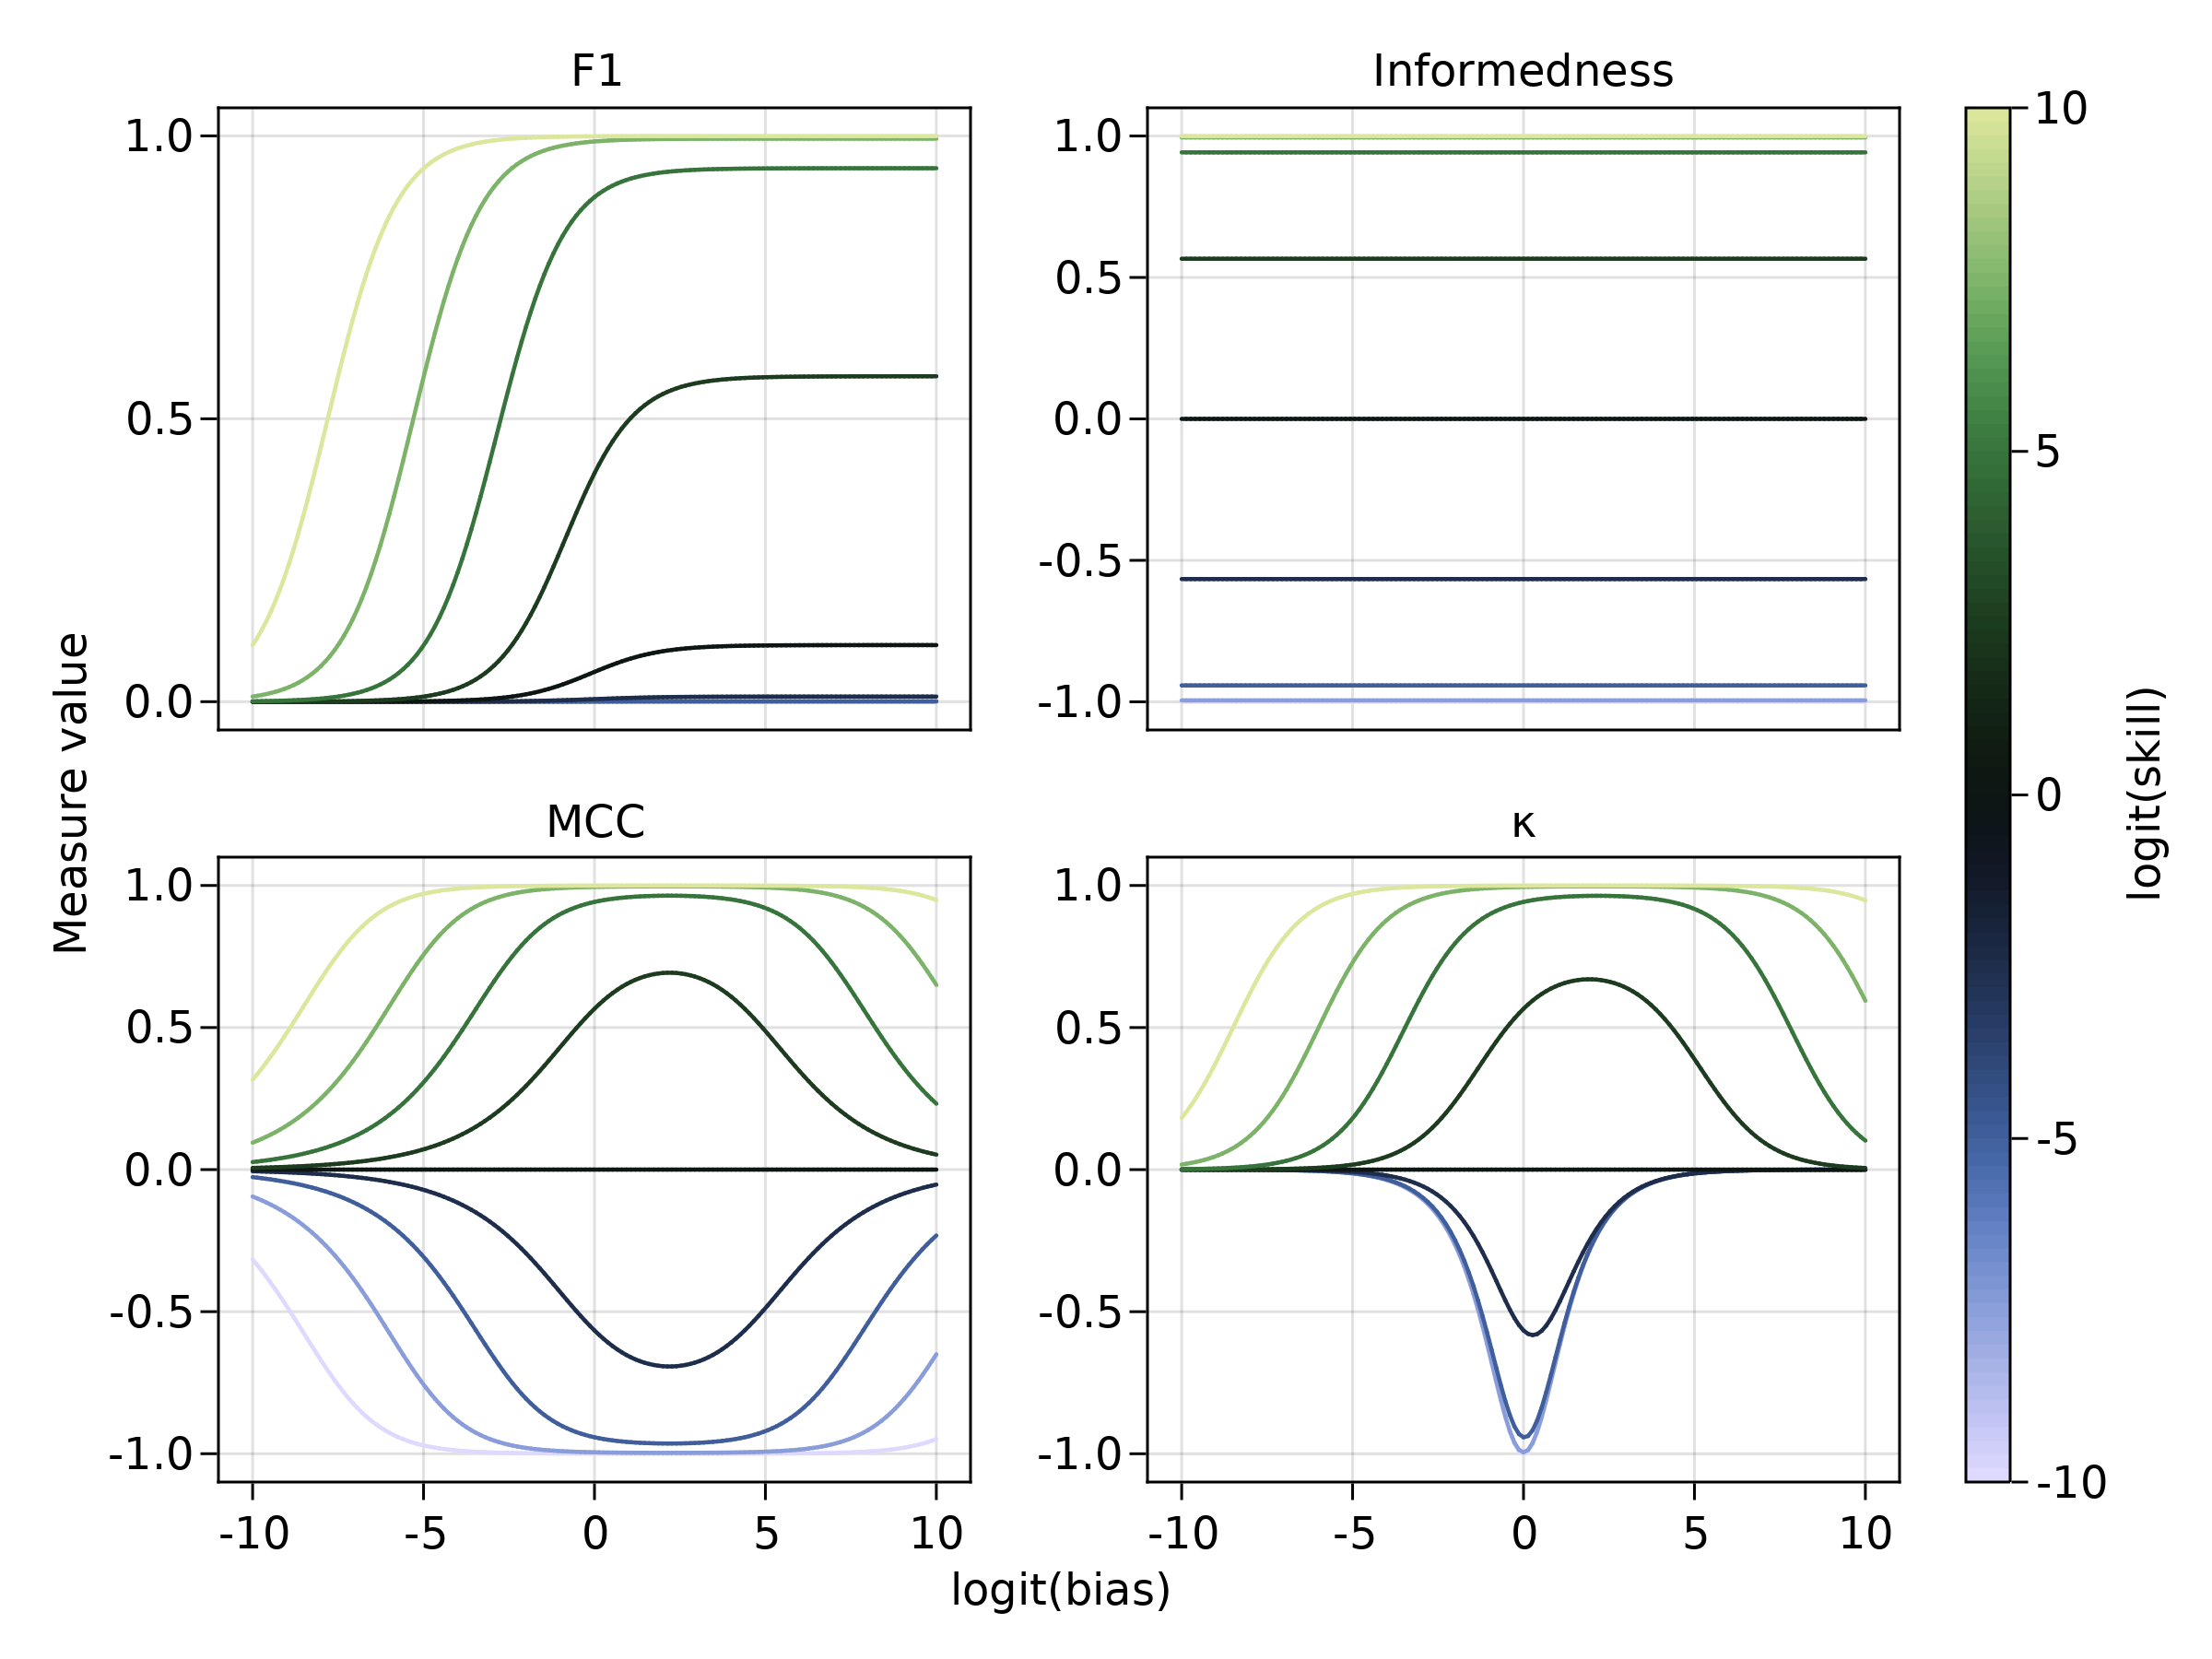
\includegraphics{figures/changing-bias.png}
\caption{Consequences of changing the classifier skills (\(s\)) and bias
(\(s\)) for a connectance \(\rho=0.15\), on accuracy, \(F_1\), postive
predictive value, and \(\kappa\). Accuracy increases with skill, but
also increases when the bias tends towards estimating \emph{fewer}
interactions. The \(F_1\) score increases with skill but also increases
when the bias tends towards estimating \emph{more} interactions; PPV
behaves in the same way. Interestingly, \(\kappa\) responds as expected
to skill (being negative whenever \(s < 0.5\)), and peaks for values of
\(b \approx 0.5\); nevertheless, the value of bias for which \(\kappa\)
is maximized in \emph{not} \(b=0.5\), but instead increases with
classifier skill. In other words, at equal skill, maximizing \(\kappa\)
would lead to select a \emph{more} biased classifier.}\label{fig:bias}
}
\end{figure}

In fig.~\ref{fig:bias}, we show that none of the four measures satisfy
all the considerations at once: \(F_1\) increases with skill, and
increases monotonously with bias; this is because \(F_1\) does not
account for true negatives, and the increase in positive detection masks
the over-prediction of interactions. Informedness varies with skill,
reaching 0 for a no-skill classifier, but is entirely unsensitive to
bias. Both MCC and \(\kappa\) have the same behavior, whereby they
increase with skill. \(\kappa\) peaks at increasing values of biass for
increasing skill, \emph{i.e.} is likely to lead to the selection of a
classifier that over-predicts interactions. By contract, MCC peaks at
the same value, regardless of skill, but this value is not
\(\text{logit}(b)=0\): unless at very high classifier skill, MCC risks
leading to a model that over-predicts interactions. In
fig.~\ref{fig:connectance}, we show that all measures except \(F_1\)
give a value of 0 for a no-skill classifier, and are forced towars their
correct maximal value when skill changes (\emph{i.e.} a more connected
networks will have higher values for a skilled classifierd, and lower
values for a classifier making mostly mistakes).

\begin{figure}
\hypertarget{fig:connectance}{%
\centering
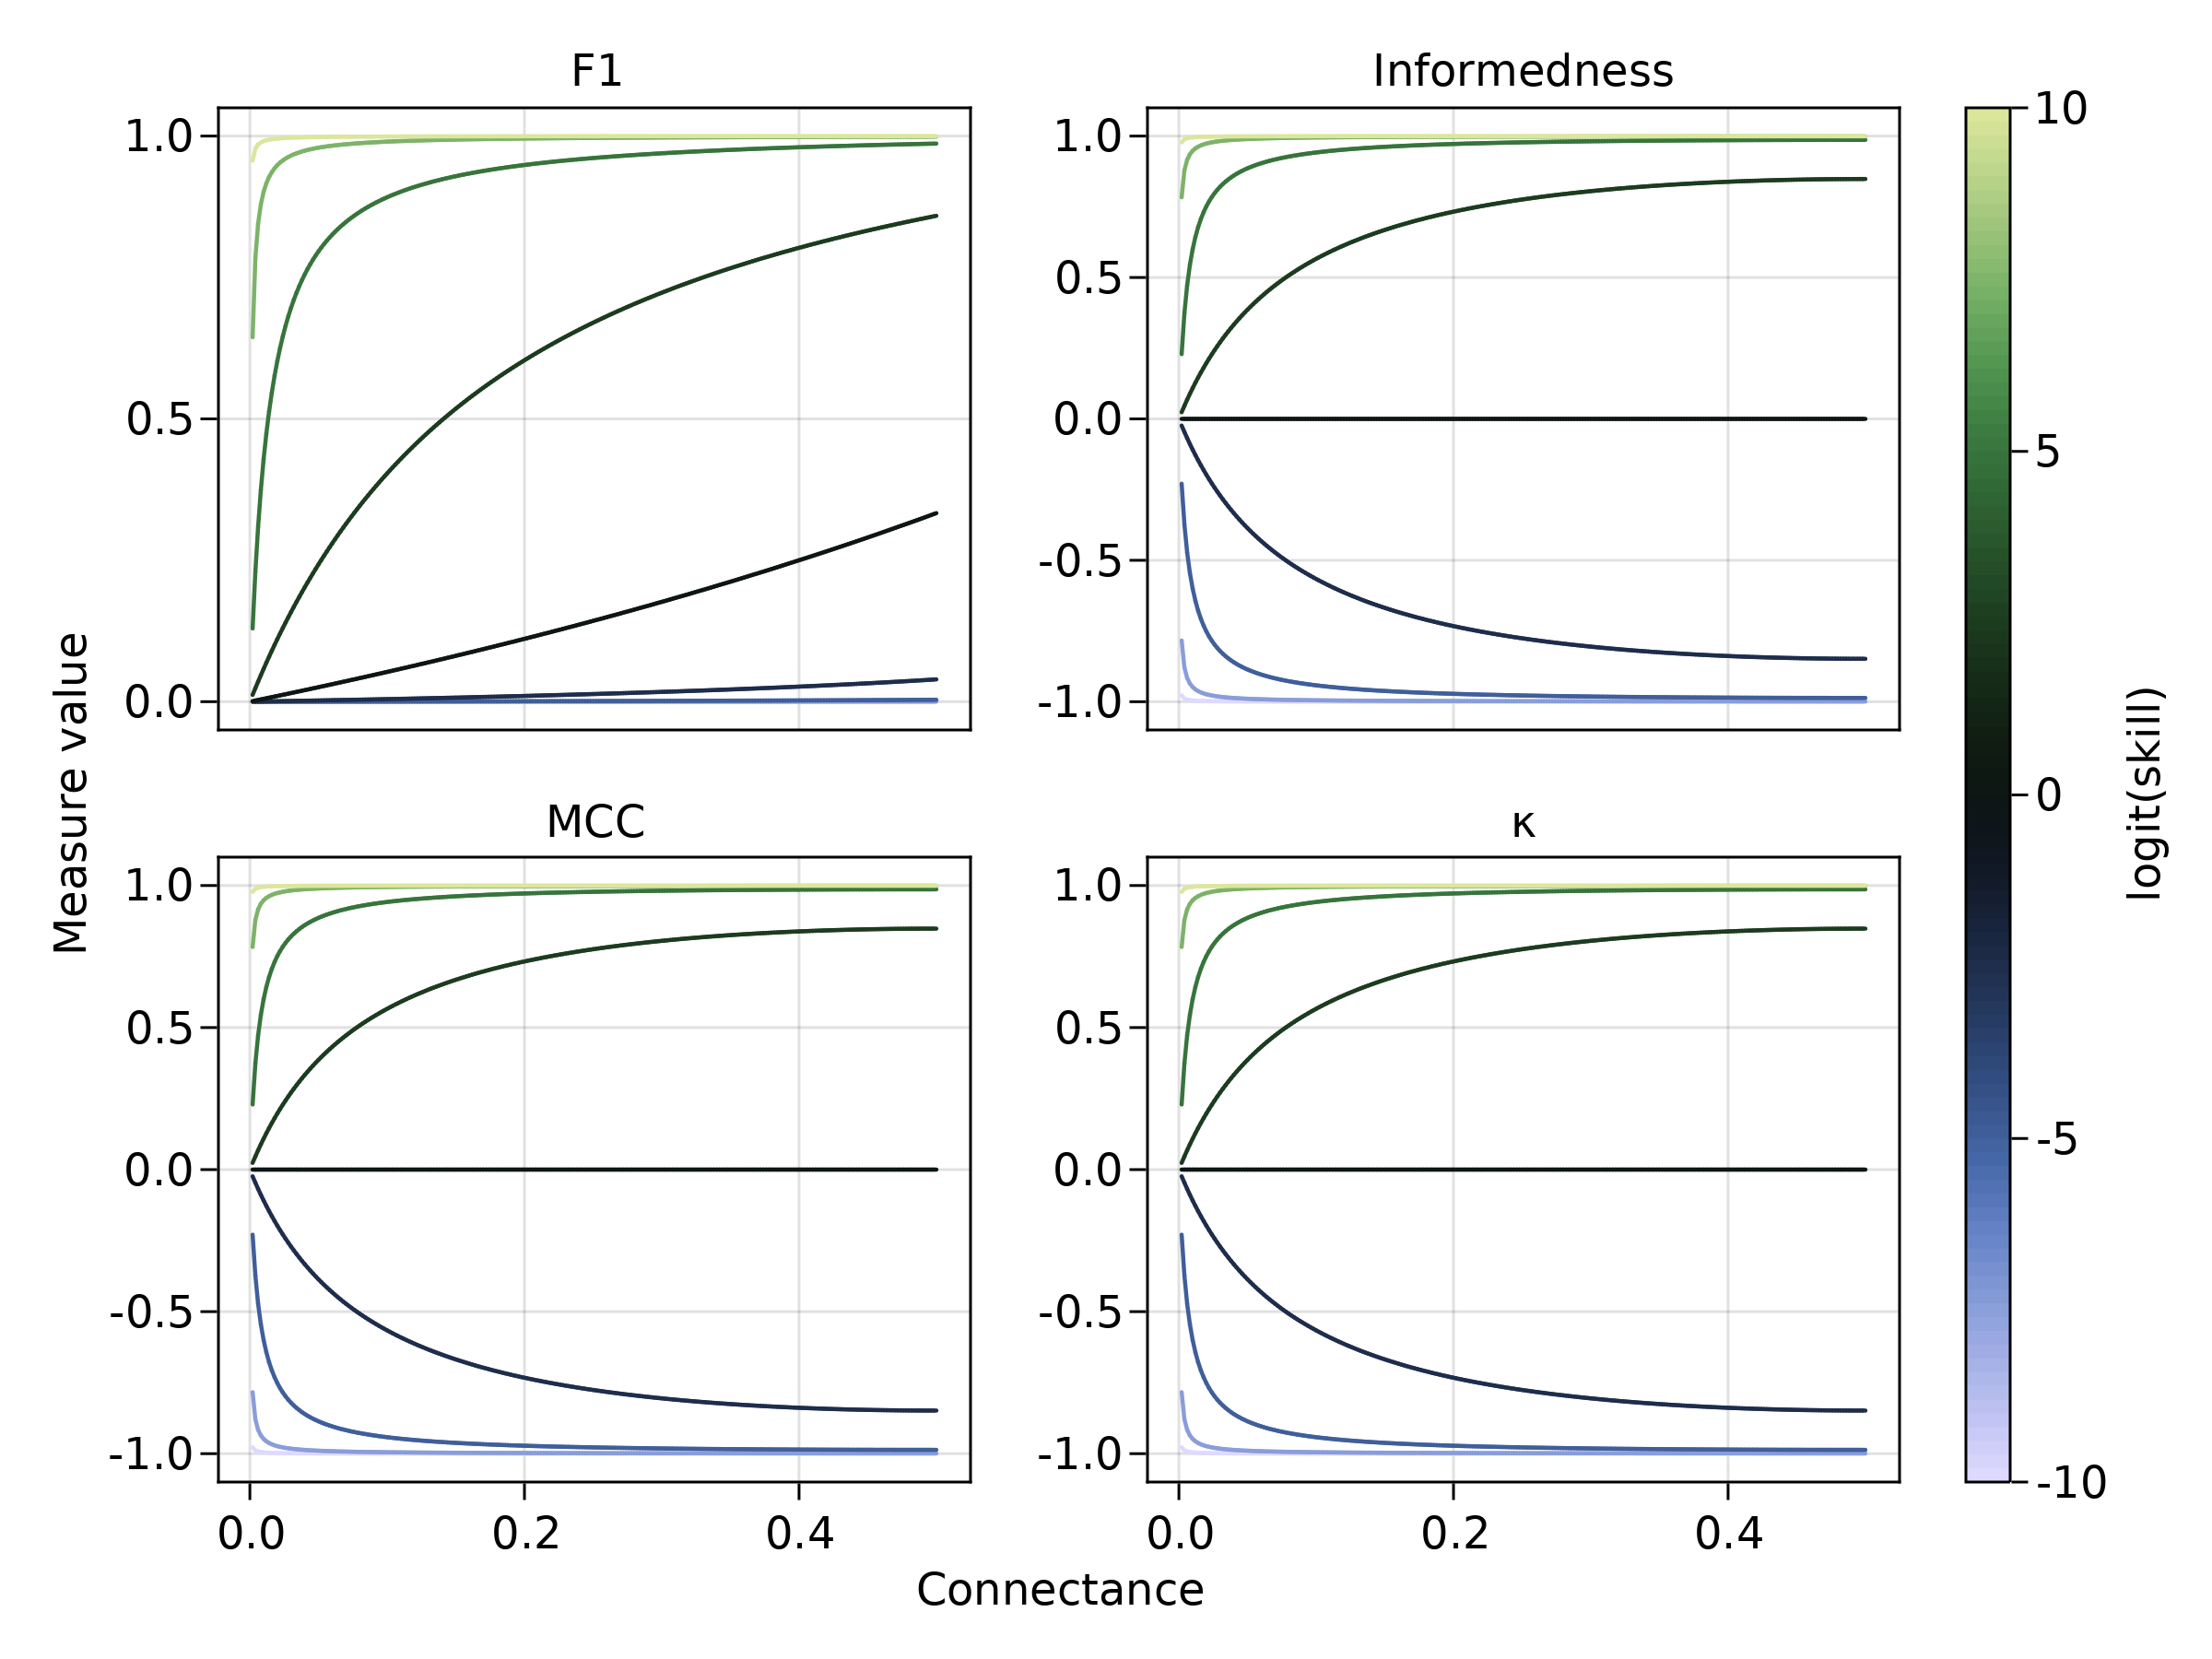
\includegraphics{figures/changing-connectance.png}
\caption{As in fig.~\ref{fig:bias}, consequences of changing connectance
for different levels of classifier skill, assuming no classifier bias.
Informedness, \(\kappa\), and MCC do increase with connectance, but only
when the classifier is not no-skill; by way of contrast, a more
connected network will give a higher \(F_1\) value even with a no-skill
classifier.}\label{fig:connectance}
}
\end{figure}

These two analyses point to the following recommendations: MCC is indeed
more appropriate than \(\kappa\), as although sensitive to bias, it is
sensitive in a consistent way. Informedness is appropriate at
discriminating between different skills, but confounded by bias. As both
of these measures bring valuable information on the model behavior, we
will retain them for future analyses. \(F_1\) is increasing with bias,
and should not be prioritized to evalue the performance of the model.
The discussion of sensitivity to bias should come with a domain-specific
caveat: although it is likely that interactions documented in ecological
networks are correct, a lot of non-interactions are simply unobserved;
as predictive models are used for data-inflation (\emph{i.e.} the
prediction of new interactions), it is not necessarily a bad thing in
practice to select models that predict more interactions than the
original dataset, because the original dataset misses some interactions.
Furthermore, the weight of positive interactions could be adjusted if
some information about the extent of undersampling exists (\emph{e.g.}
Branco et al., 2015). In a recent large-scale imputation of interactions
in the mammal-virus networks, Poisot et al. (2021) for example estimated
that 93\% of interactions are yet to be documented.

\hypertarget{numerical-experiments-on-training-strategy}{%
\section{Numerical experiments on training
strategy}\label{numerical-experiments-on-training-strategy}}

In the following section, we will generate random bipartite networks
(this works without loss of generality on unipartite networks), and
train four binary classifiers (as well as an ensemble model using the
sum of ranged outputs from the component models) on 30\% of the
interaction data. In practice, testing usually uses 70\% of the total
data; for ecological networks, where interactions are sparse \emph{and}
the number of species is low, this may not be the best solution, as the
testing set becomes constrained not by the \emph{proportion} of
interactions, but by their \emph{number}. Preliminary experiments using
different splits revealed no qualitative change in the results. Networks
are generated by picking a random infectiousness trait \(v_i\) for 100
species (from a beta distribution \(B(\alpha=6,\beta=8)\) distribution),
and a resistance trait \(h_j\) for 100 species (from
\(B(\alpha=2,\beta=8)\) distribution). There is an interaction between
\(i\) and \(j\) when \(v_i-\xi/2 \le h_j \le v_i+\xi/2\), where \(\xi\)
is a constant regulating the connectance of the network (there is an
almost 1:1 relationship between \(\xi\) and connectance), and varies
uniformly in \([0.05, 0.35]\). This model gives fully interval networks
that are close analogues to the bacteria--phage model of Weitz et al.
(2005), with both a modular structure and a non-uniform degree
distribution. This dataset is easy for almost any algorithm to learn:
when trained with features \([v_i, h_j, \text{abs}(v_i, h_j)] ^T\) to
predict the interactions between \(i\) and \(j\), all four models
presented below were able to reach almost perfect predictions all the
time (data not presented here) -- this is in part because the rule
(there is maximum value of the distance between traits for which there
is an interaction) is fixed for all interactions. In order to make the
problem more difficult to solve, we use \([v_i, h_j]\) as a feature
vector (\emph{i.e.} the traits on which the models are trained), and
therefore the models will have to uncover that the rule for interaction
is \(\text{abs}(v_i, h_j) \le \xi\). The models therefore all have the
form

\[
\begin{bmatrix}
           x_{1} \\
           x_{2} \\
           \vdots \\
           x_{m}
         \end{bmatrix}
\]

The training sample is composed of 30\% of the \(10^4\) possible entries
in the network, \emph{i.e.} \(n=3000\). Out of these interactions, we
pick a proportion \(\nu\) (the training set bias) to be positive, so
that the training set has \(\nu n\) interactions, and \((1-\nu) n\)
non-interactions. We vary \(\nu\) uniformly in \(]0,1[\). This allows to
evaluate how the measures of binary classification performance respond
to artificially rebalanced dataset for a given network connectance. The
rest of the dataset (\(n=7000\) pairs of species) is used as a testing
set, on which all furher measures are calculated. Note that although the
training set is balanced, the testing set is not, and retains (part of)
the imbalance of the original data.

The dataset used for numerical experiments is composed of 64000 such
\((\xi, \nu)\) pairs, on which four machines are trained: a decision
tree regressor, a boosted regression tree, a ridge regressor, and a
random forest regressor. All models were taken from the \texttt{MLJ.jl}
package (Blaom et al., 2020; Blaom \& Vollmer, 2020) in Julia 1.7
(Bezanson et al., 2017). All machines use the default parameterization;
this is an obvious deviation from best practices, as the hyperparameters
of any machine require training before its application on a real
dataset. As we use 64000 such datasets, this would require 256000 unique
instances of tweaking the hyperparameters, which is not realistic.
Therefore, we assume that the default parameterizations are comparable
across networks. All machines return a quantitative prediction, usually
(but not necessarily) in \([0,1]\), which is proportional (but not
necessarily linearly) to the probability of an interaction between \(i\)
and \(j\).

In order to pick the best adjacency matrix for a given trained machine,
we performed a thresholding approach using 500 steps on predictions from
the testing set, and picking the threshold that maximized Youden's
informedness, which is usually the optimized target for imbalanced
classification. During the thresholding step, we measured the area under
the receiving-operator characteristic (ROC-AUC) and precision-recall
(PR-AUC) curves, as measures of overall performance over the range of
returned values. We report the ROC-AUC and PR-AUC, as well as a suite of
other measures as introduced in the next section, for the best
threshold. The ensemble model was generated by summing the predictions
of all component models on the testing set (ranged in \([0,1]\)), then
put through the same thresholding process. The complete code to run the
simulations is given as an appendix; running the final simulation
required 4.8 core days (approx. 117 hours).

After the simulations were completed, we removed all runs (\emph{i.e.}
pairs of \(\xi\) and \(\nu\)) for which at least one of the following
conditions was met: the accuracy was 0, the true positive or true
negative rates were 0, the connectance was larger than 0.25. This
removes both the obviously failed model runs, and the networks that are
more densely connected compared to the connectance of empirical food
webs (and are therefore less difficult to predict, being less
imbalanced; preliminary analyses of data with a connectance larger than
3 revealed that all machines reached consistently high performance).

\hypertarget{effect-of-training-set-bias-on-performance}{%
\subsection{Effect of training set bias on
performance}\label{effect-of-training-set-bias-on-performance}}

In fig.~\ref{fig:biasmccinf}, we present the response of MCC and
informedness to (i) five levels of network connectance and (ii) a
gradient of training set bias, for the four component models as well as
the ensemble. All models reached a higher performance on more connected
networks, and using more biased training sets (with the exception of
ridge regression, whose informedness decreased in performance with
training set bias). In all cases, informedness was extremely high, which
is an expected consequence of the fact that this is the value we
optimized to determine the cutoff. MCC increased with training set bias,
although this increase became less steep with increasing connectance.
Interestingly, the ensemble almost always outclassed its component
models. In a few cases, both MCC and informedness stared decreasing when
the training set bias got too close to one, which suggests that it is
possible to over-correct the imbalance.

\begin{figure}
\hypertarget{fig:biasmccinf}{%
\centering
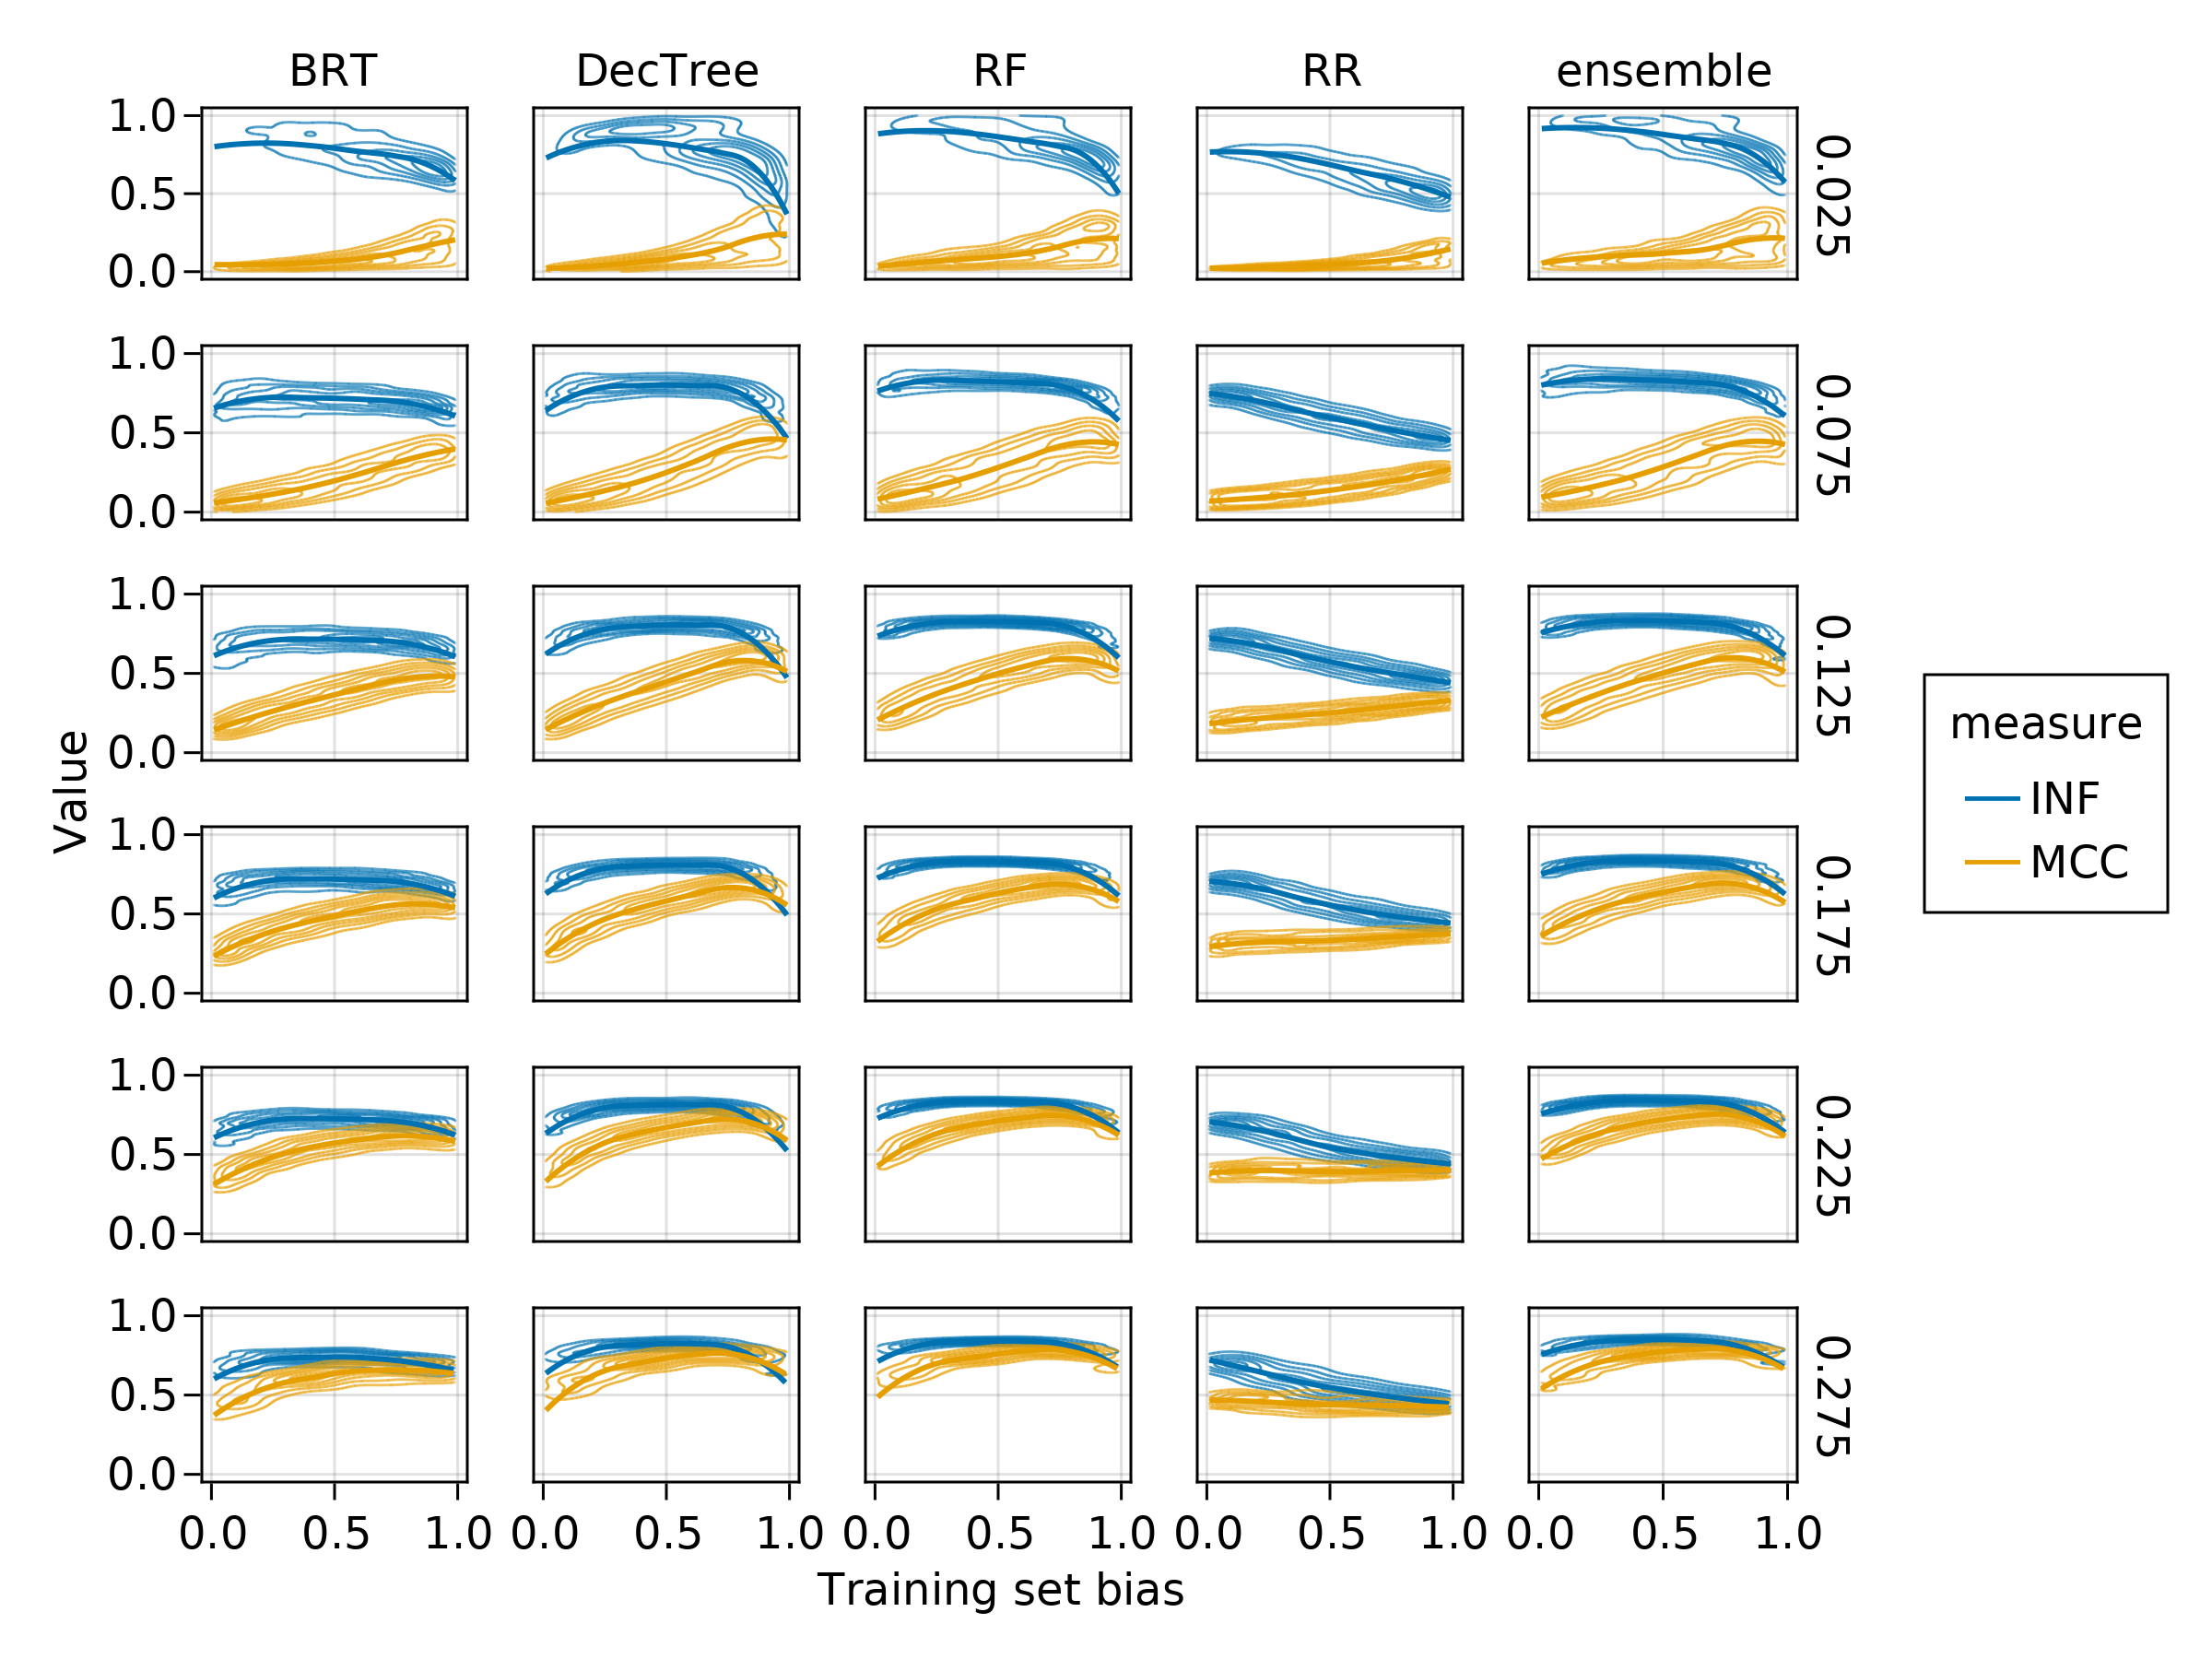
\includegraphics{figures/bias_mcc_inf.png}
\caption{Response of MCC and Informedness to changes in the training set
bias for a fixed connectance (rows). Both of these values approach 1 for
a good model. Informedness is consistently high, and by contrast, MCC
increases with additional training set bias. Across all models, training
on a more connected network is easier.}\label{fig:biasmccinf}
}
\end{figure}

In fig.~\ref{fig:biasrocpr}, we present the same information as
fig.~\ref{fig:biasmccinf}, this time using ROC-AUC and PR-AUC. ROC-AUC
is always high, and does not vary with training set bias. On the other
hand, PR-AUC shows very strong responses, increasing with training set
bias. It is notable here that two classifiers that seemed to be
performing well (Decision Tree and Random Forest) based on their MCC are
not able to reach a high PR-AUC even at higher connectances. As in
fig.~\ref{fig:biasmccinf}, the ensemble outperforms its component
models.

\begin{figure}
\hypertarget{fig:biasrocpr}{%
\centering
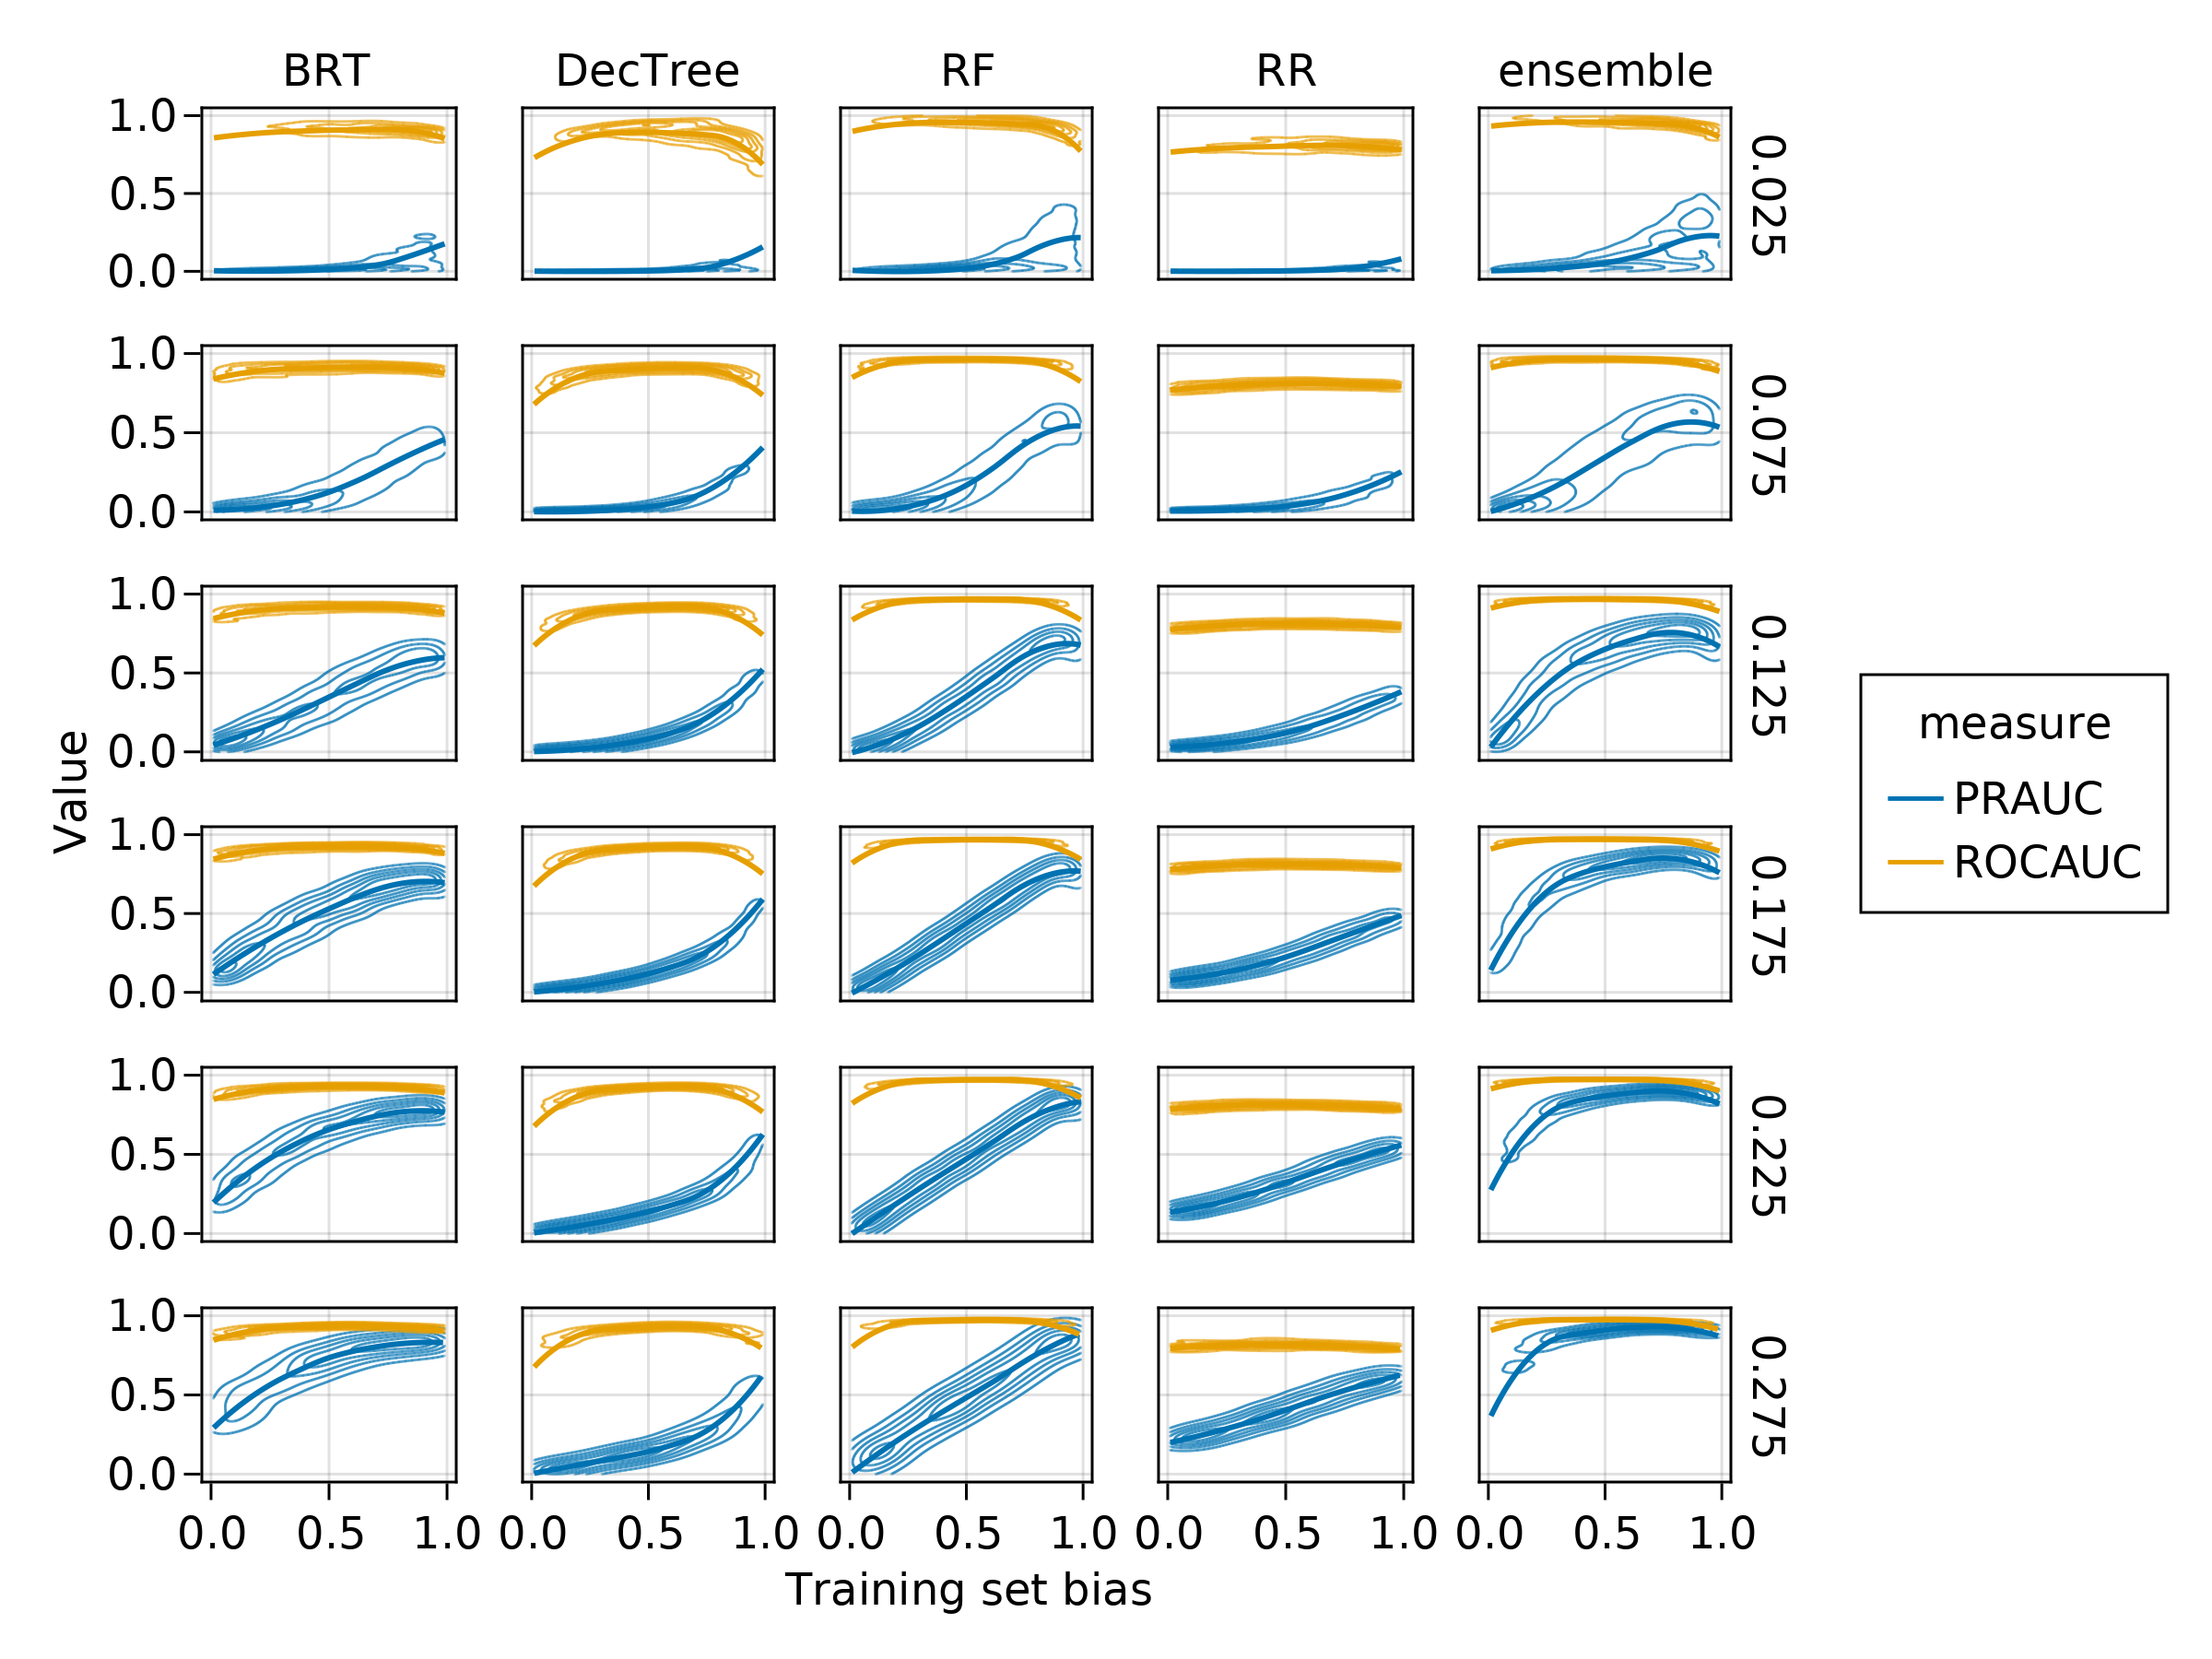
\includegraphics{figures/bias_roc_pr.png}
\caption{Response of ROC-AUC and PR-AUC to changes in the training set
bias for a fixed connectance (rows). ROC-AUC is consistently high, and
therefore not properly able to separate good from poor classifiers. On
the other hand, PR-AUC responds to changes in the training set. As in
fig.~\ref{fig:biasmccinf}, training on more connected networks is
easier.}\label{fig:biasrocpr}
}
\end{figure}

Based on the results presented in fig.~\ref{fig:biasmccinf} and
fig.~\ref{fig:biasrocpr}, it seems that informedness and ROC-AUC are not
necessarily able to discriminate between good and bad classifiers
(although this result may be an artifact for informedness, as it has
been optimized when thresholding). On the other hand, MCC and PR-AUC
show a strong response to training set bias, and may therefore be more
useful at model comparison.

\hypertarget{required-amount-of-positives-to-get-the-best-performance}{%
\subsection{Required amount of positives to get the best
performance}\label{required-amount-of-positives-to-get-the-best-performance}}

The previous results revealed that the measure of classification
performance responds both to the bias in the training set \emph{and} to
the connectance of the network; from a practical point of view,
assembling a training set requires to withold positive information,
which in ecological networks are very scarce (and typically more
valuable than negatives, on which there is a doubt). For this reason,
across all values of connectance, we measured the training set bias that
maximized a series of performance measures. When this value is high, the
training set needs to skew more positive in order to get a performant
model; when this value is about 0.5, the training set needs to be
artificially balanced to optimize the model performance. These results
are presented in fig.~\ref{fig:optimbias}.

\begin{figure}
\hypertarget{fig:optimbias}{%
\centering
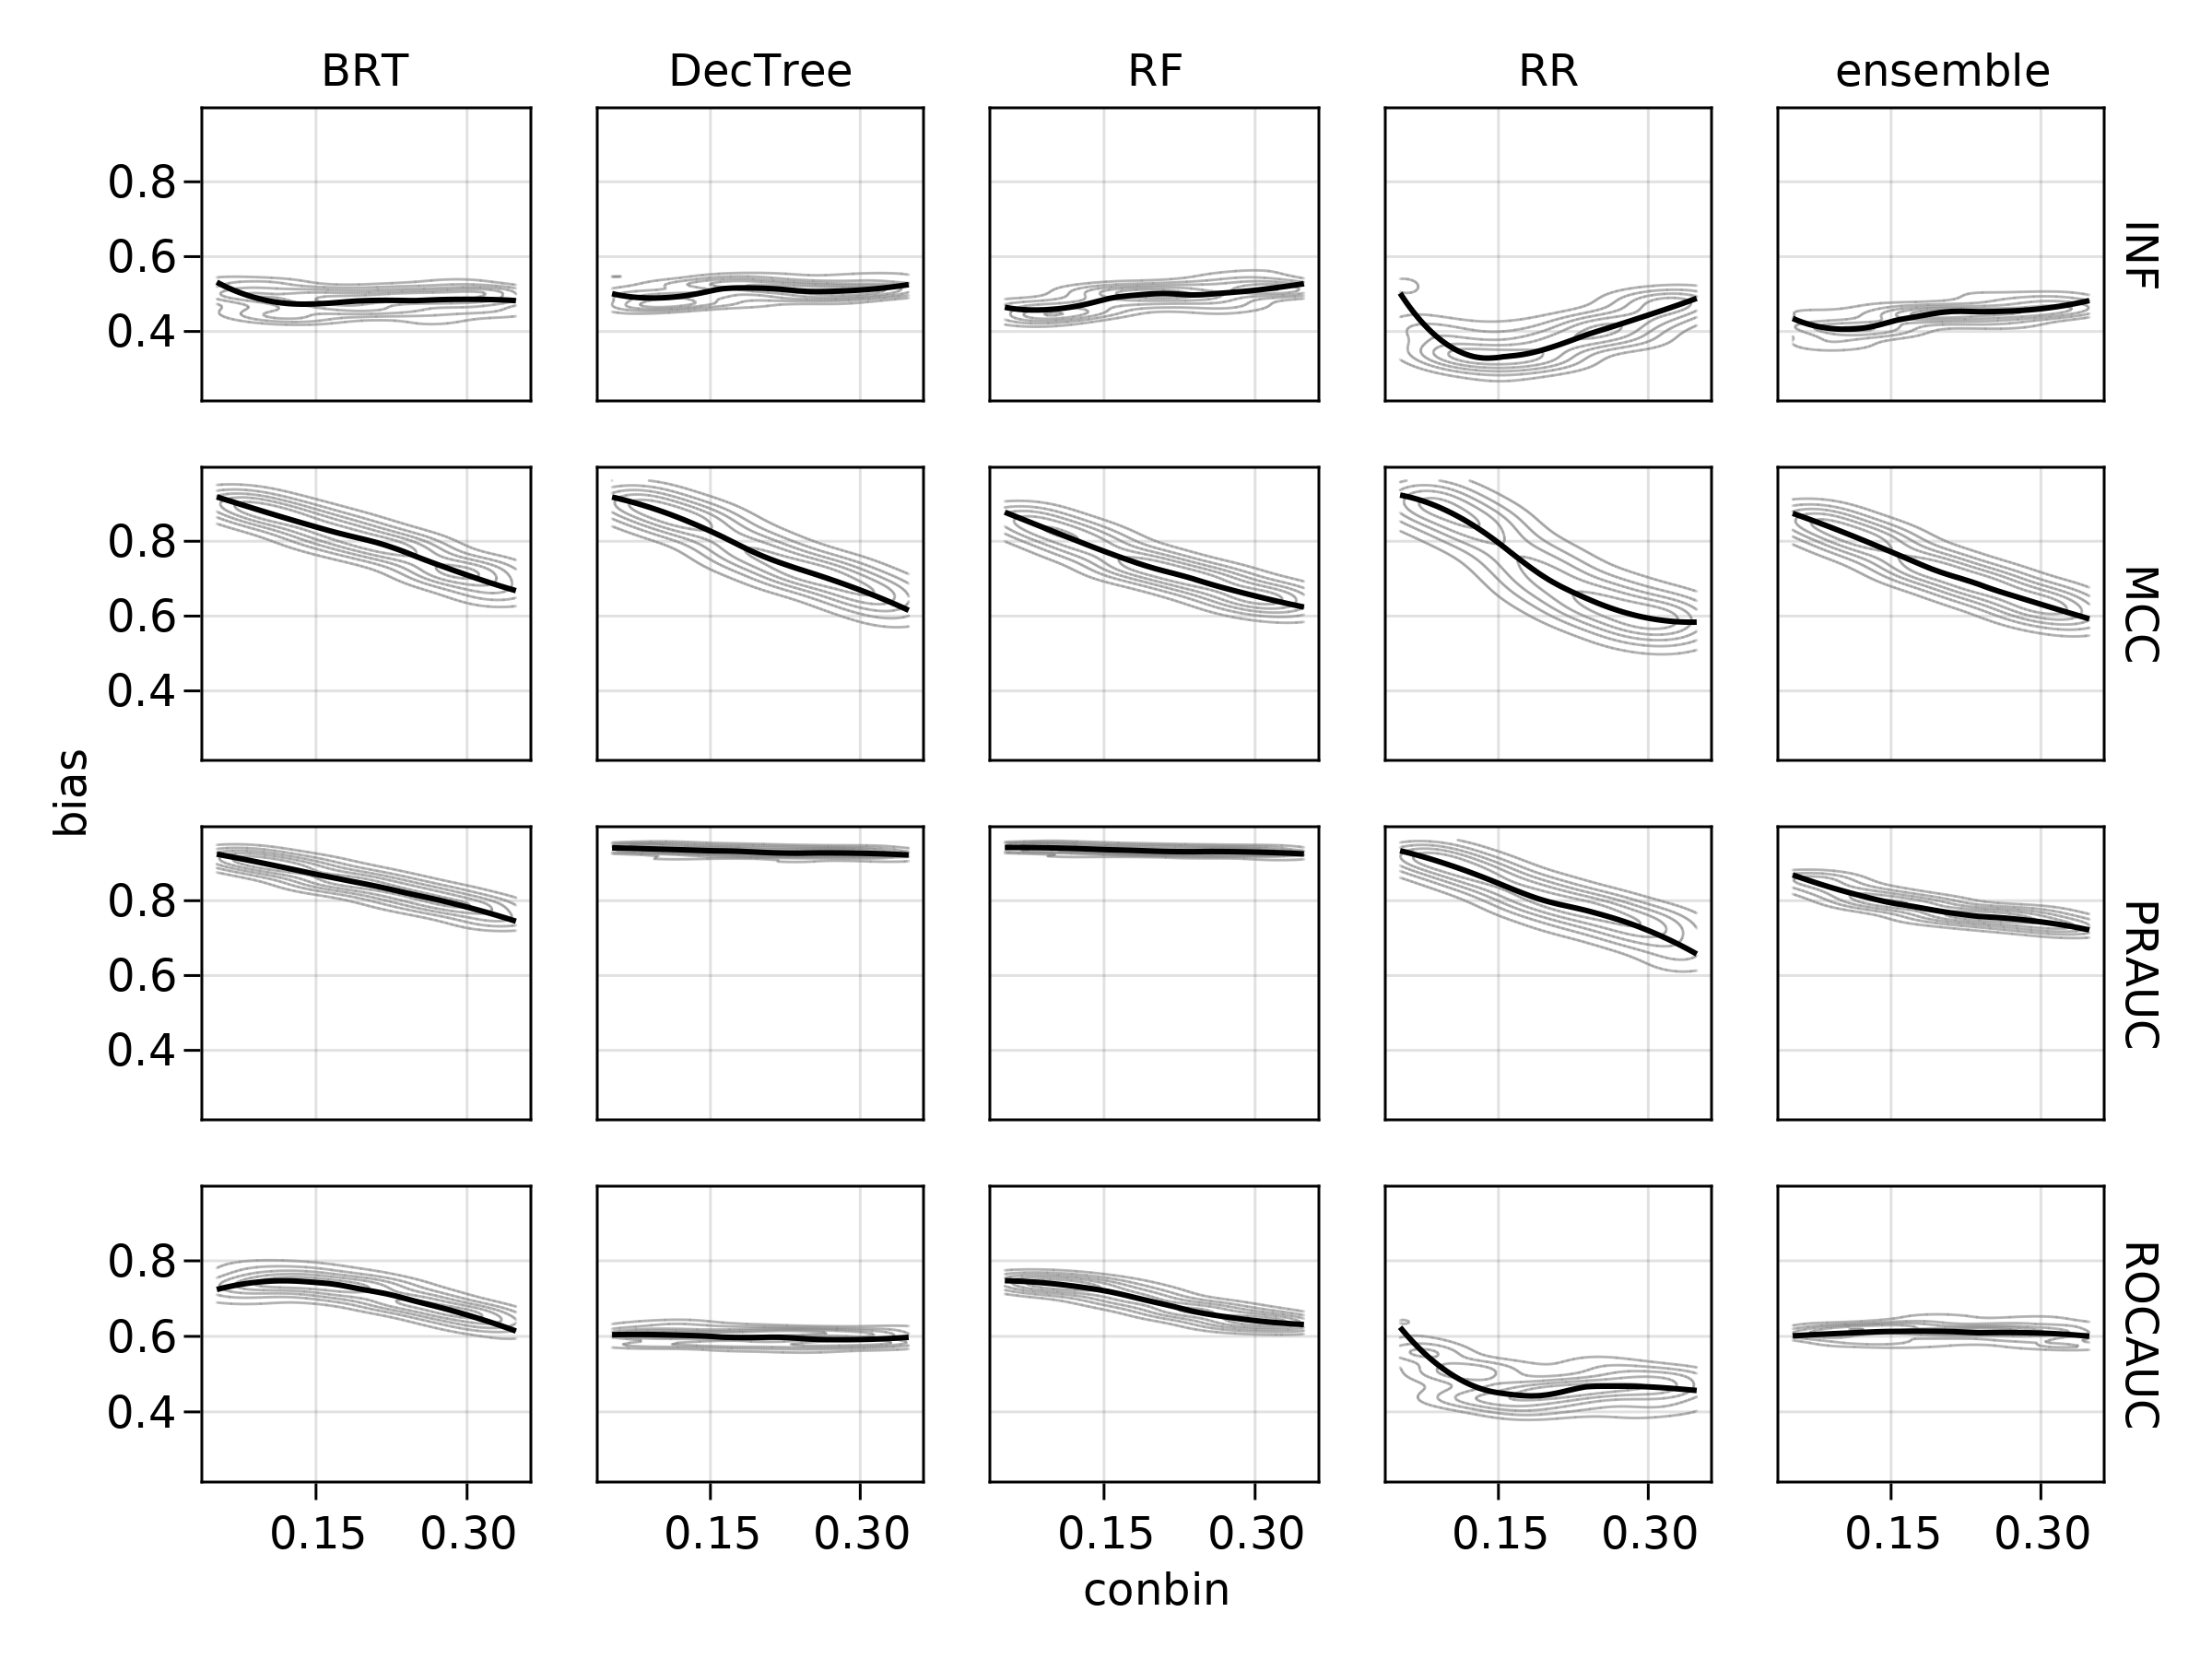
\includegraphics{figures/optim_bias.png}
\caption{Value of the optimal training set bias for the different models
and measures evaluated here, over a range of connectances. Informedness
was reliably maximized for balanced training sets, and kept this
behavior across models. For other measures, larger connectances in the
true network allowed lower biases in the training set. In a large number
of cases, ``over-correcting'' by having training sets with more than
half instances representing interactions would maximize the values of
the model performance measures.}\label{fig:optimbias}
}
\end{figure}

The more ``optimistic'' measures (ROC-AUC and informedness) required a
biasing of the dataset from about 0.4 to 0.75 to be maximized, with the
amount of bias required decreasing only slightly with the connectance of
the original network. MCC and PR-AUC required values of training set
bias from 0.75 to almost 1 to be optimized, which is in line with the
results of the previous section, \emph{i.e.} they are more stringent
tests of model performance. These results suggest that learning from a
dataset with very low connectance can be a different task than for more
connected networks: it becomes increasingly important to caputre the
mechanisms that make an interaction \emph{exist}, and therefore having a
slightly more biased training dataset might be beneficial. As
connectance increases, the need for biased training sets is less
prominent, as learning the rules for which interactions \emph{do not}
exist starts gaining importance.

\begin{figure}
\hypertarget{fig:optimperf}{%
\centering
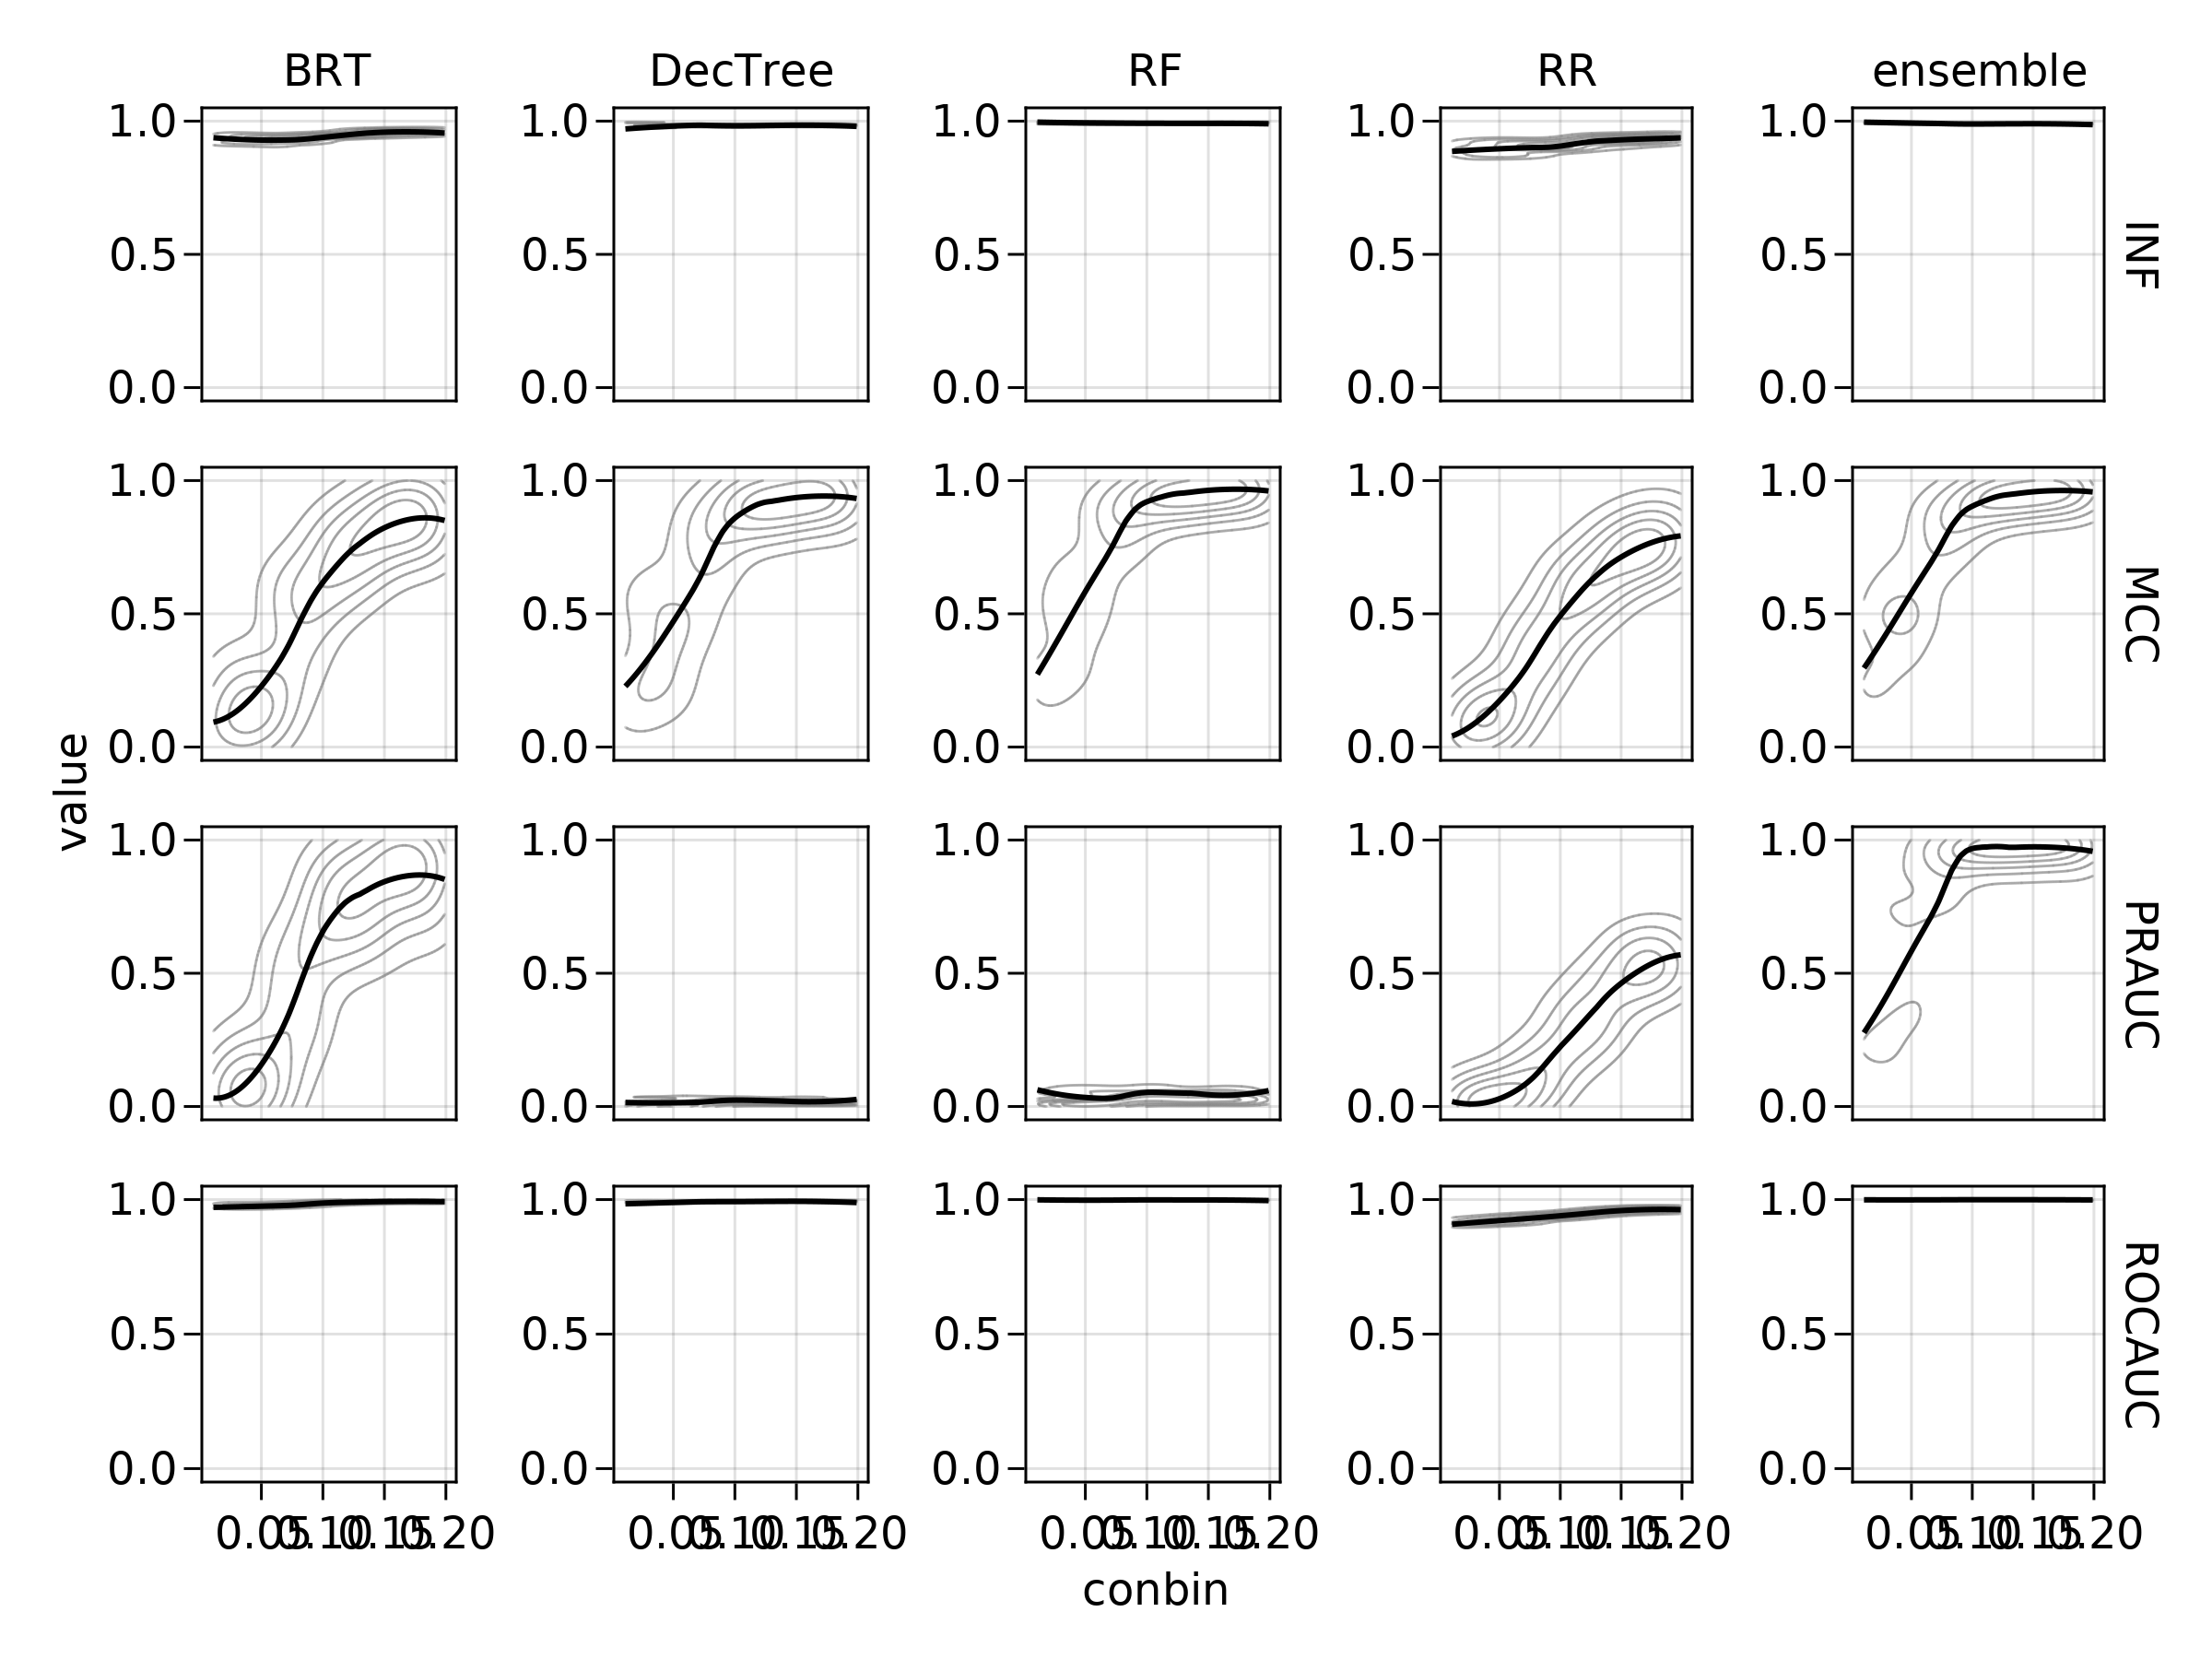
\includegraphics{figures/optim_perf.png}
\caption{When trained on their optimally biased training set, most
models were able to maximize their performance; this is not true for
decision tree, which had a very low PR-AUC, and to some extent for ridge
regression who had a slow increase with network connectance. The
ensemble had a consistently high performance despite incorporating poor
models.}\label{fig:optimperf}
}
\end{figure}

When trained at their optimal training set bias, connectance still had a
significant impact on the performance of some machines
fig.~\ref{fig:optimperf}. Notably, Decision Tree, Random Forest, and
Ridge Regression had low values of PR-AUC. In all cases, the Boosted
Regression Tree was reaching very good predictions (esepcially for
connectances larger than 0.1), and the ensemble was almost always
scoring perfectly. This suggests that all the models are biased in
different ways, and that the averaging in the ensemble is able to
correct these biases. We do not expect this last result to have any
generality, and provide a discussion of a recent exemple in which the
ensemble was performing worse than its components models.

\hypertarget{do-better-classification-accuracy-result-in-more-realistic-networks}{%
\section{Do better classification accuracy result in more realistic
networks?}\label{do-better-classification-accuracy-result-in-more-realistic-networks}}

In this last section, we generate a network using the same model as
before, with \(S_1, S_2 = 50, 80\) species, a connectance of
\(\approx 0.16\) (\(\xi = 0.19\)), and a training set bias of \(0.7\).
The prediction made on the complete dataset is presented in
fig.~\ref{fig:ecovalid}. Visualizing the results this way highlights the
importance of exploratory data analysis: whereas all models return a
network with interactions laying mostly on the diagonal (as expected),
the Ridge Regression is quite obviously biased. Despite this, we can see
that the ensemble is close to the initial dataset.

\begin{figure}
\hypertarget{fig:ecovalid}{%
\centering
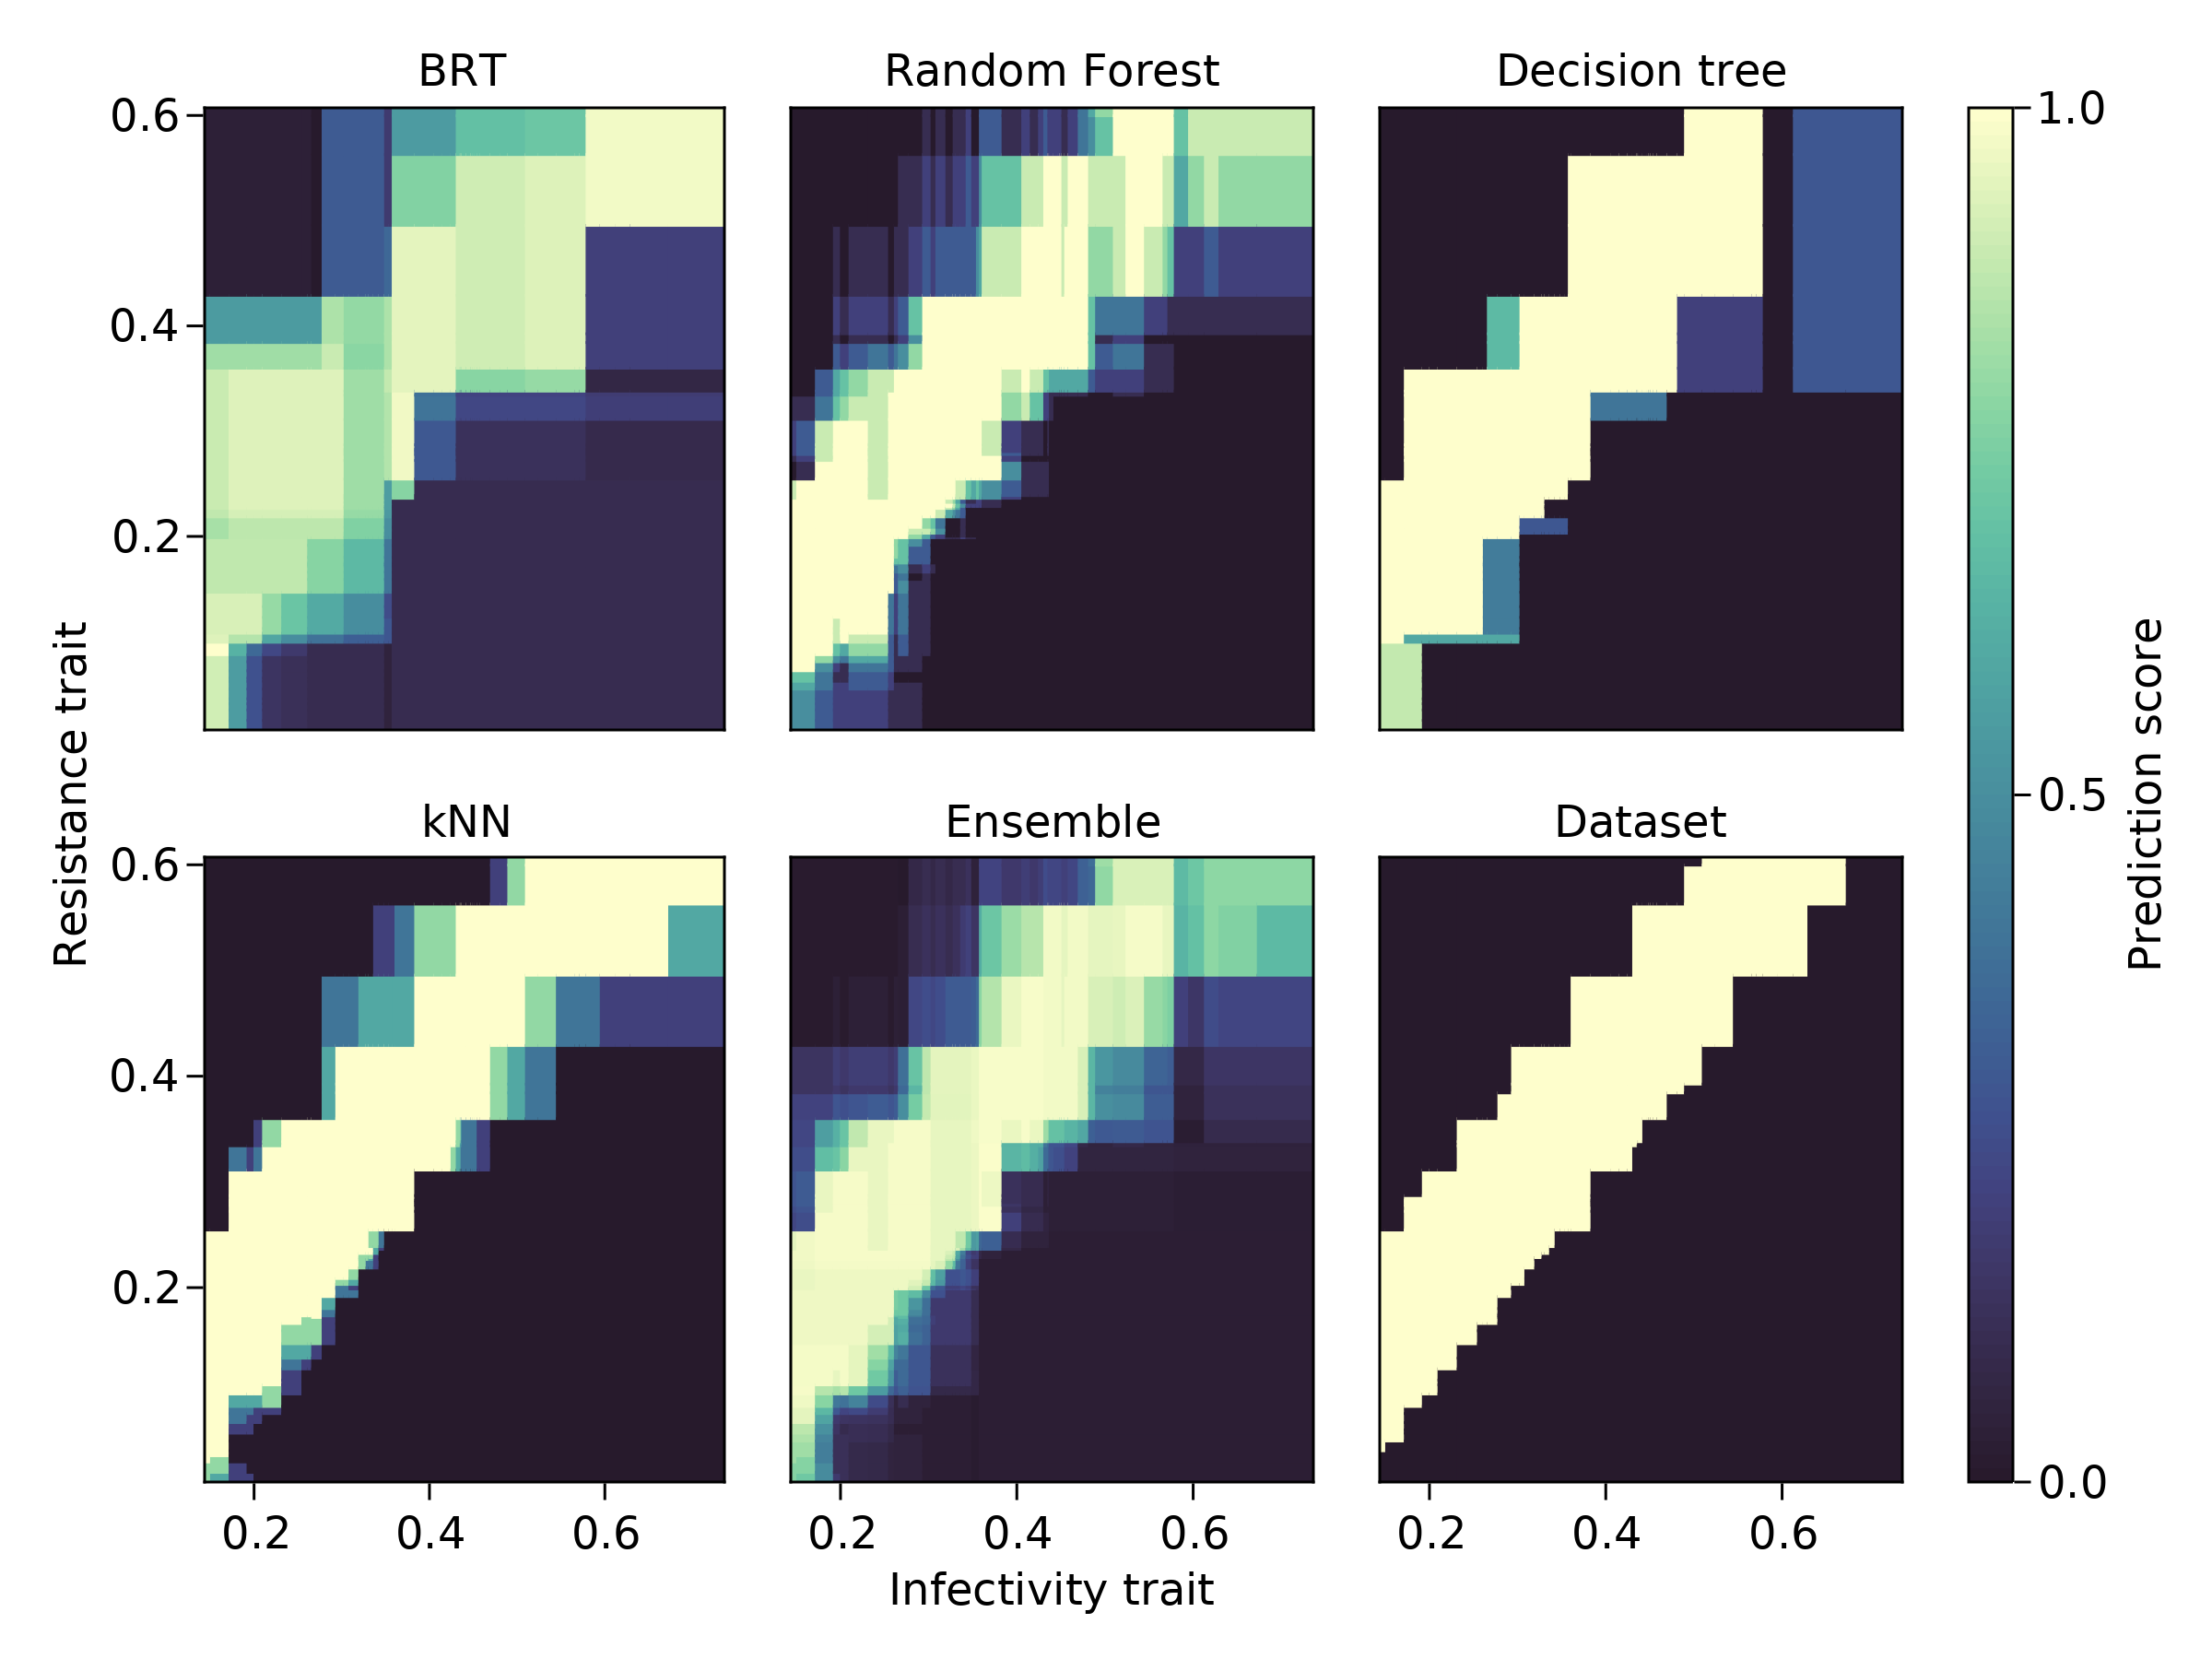
\includegraphics{figures/valid_ensemble.png}
\caption{Visualisation of the models predictions for one instance of a
network prediction problem (shown in the ``Dataset'' panel). This figure
reveals how inspecting the details of the prediction is important:
indeed, although the performance measures hint at the fact that ridge
regression is mediocre, this figure reveals that it is making
predictions that correspond to a network with an entirely different
topology (namely, nested as opposed to diagonal).}\label{fig:ecovalid}
}
\end{figure}

The trained models were then thresholded (again by optimising
informedness), and their predictions transformed back into networks for
analysis; specifically, we measured the connectance, nestedness (REF),
and modularity (REF). This process was repeated 250 times, and the
results are presented in tbl.~\ref{tbl:comparison}. The random forest
model is an interesting instance here: it produces the network that
looks the most like the original dataset, despite having a very low
PR-AUC, suggesting it hits high recall at the cost of low precision.
Although the ensemble was able to reach a very high PR-AUC (and a very
high ROC-AUC), this did not necessarily translate into more accurate
reconstructions of the structure of the network. This result bears
elaborating. Measures of model performance capture how much of the
interactions and non-interactions are correctly identified. As long as
these predictions are not perfect, some interactions will be predicted
at the ``wrong'' position in the network; these measures cannot describe
the structural effect of these mistakes. On the other hand, measures of
network structure can have the same value with interactions that fall at
drastically different positions; this is in part because a lot of these
measures covary with connectance, and in part because as long as these
values are not 0 or their respective maximum, there is a large number of
network configurations that can have the same value. That ROC-AUC is
consistently larger than PR-AUC may be a case of this measure masking
models that are not, individually, strong predictors (Jeni et al.,
2013).

\hypertarget{tbl:comparison}{}
\begin{longtable}[]{@{}rccccccc@{}}
\caption{\label{tbl:comparison}Values of four performance metrics, and
three network structure metrics, for 250 independent predictions similar
to the ones presented in fig.~\ref{fig:ecovalid}. The values in
\textbf{bold} indicate the best value for each column (including ties).
Because the values have been rounded, values of 1.0 for the ROC-AUC
column indicate an average \(\ge 0.99\).}\tabularnewline
\toprule
Model & MCC & Inf. & ROC-AUC & PR-AUC & Conn. & \(\eta\) &
\(Q\)\tabularnewline
\midrule
\endfirsthead
\toprule
Model & MCC & Inf. & ROC-AUC & PR-AUC & Conn. & \(\eta\) &
\(Q\)\tabularnewline
\midrule
\endhead
Decision tree & 0.85 & 0.92 & 0.97 & 0.12 & 0.21 & 0.76 &
0.31\tabularnewline
BRT & \textbf{0.90} & 0.90 & 0.98 & 0.86 & 0.23 & 0.82 &
0.27\tabularnewline
Random Forest & \textbf{0.90} & \textbf{0.96} & \textbf{1.00} & 0.27 &
\textbf{0.20} & \textbf{0.72} & \textbf{0.32}\tabularnewline
Ridge Regression & 0.80 & 0.91 & 0.95 & 0.58 & 0.24 & 1.0 &
0.18\tabularnewline
Ensemble & 0.88 & 0.94 & \textbf{1.00} & \textbf{0.96} & \textbf{0.20} &
0.75 & 0.31\tabularnewline
Data & & & & & 0.18 & 0.66 & 0.34\tabularnewline
\bottomrule
\end{longtable}

\hypertarget{guidelines-for-the-assesment-of-network-predictive-models}{%
\section{Guidelines for the assesment of network predictive
models}\label{guidelines-for-the-assesment-of-network-predictive-models}}

The results presented here highlight an interesting paradox: although
the Random Forest was ultimately able to get a correct estimate of
network structure tbl.~\ref{tbl:comparison}, it ultimately remains a
poor classifier, as evidenced by its low PR-AUC. This suggests that the
goal of predicting \emph{interactions} and predicting \emph{networks}
may not be solvable in the same way -- of course a perfect classifier of
interactions would make a perfect network prediction; but even the best
scoring predictor of interactions (the ensemble model) had not
necessarily the best prediction of network structure. The tasks of
predicting networks structure and of predicting interactions within
networks are essentially two different ones. For some applications
(\emph{.e.g.} comparison of network structure across gradients), one may
care more about a robust estimate of the structure, at the cost at
putting some interactions at the wrong place. For other applications
(\emph{e.g.} identifying pairs of interacting species), one may
conversely care more about getting as many pairs right, even though the
mistakes accumulate in the form of a slightly worse estimate of network
structure. How these two approaches can be reconciled is undoubtedly a
task for further research. Despite this apparent tension at the heart of
the predictive exercise, we can use the results presented here to
suggest a number of guidelines.

First, because we should have more trust in reported interactions than
in reported absences of interactions, we can draw on previous literature
to recommend informedness as a measure to decide on a threshold (Chicco
et al., 2021); this being said, because informedness is insensitive to
bias, the model performance is better evaluated through the use of MCC
fig.~\ref{fig:biasmccinf}. Because \(F_1\) is monotonously sensitive to
classifier bias fig.~\ref{fig:bias} and network connectance
fig.~\ref{fig:connectance}, MCC should be prefered as a measure of model
evaluation.

Second, because the PR-AUC responds more to network connectance
fig.~\ref{fig:optimperf} and training set imbalance
fig.~\ref{fig:biasrocpr}, it should be used as a measure of model
performance over the ROC-AUC. This is not to say that ROC-AUC should be
discarded (in fact, a low ROC-AUC is a sign of an issue with the model),
but that its interpretation should be guided by the PR-AUC value.
Specifically, a high ROC-AUC is not informative, as it can be associated
to a low PR-AUC (see \emph{e.g.} Random Forest in
tbl.~\ref{tbl:comparison}) This again echoes recommendations from other
fields (Jeni et al., 2013; Saito \& Rehmsmeier, 2015).

Thirdly, regardless of network connectance, maximizing informedness
required a training set bias of about 0.5, and maximizing the MCC
required a training set bias of 0.7 and more. This has an important
consequence in ecological networks, for which the pool of positive cases
(interactions) to draw from is typically small: the most parsimonious
measure (\emph{i.e.} the one requiring to discard the least amount of
information to train the model) will give the best validation potential,
and is probably the informedness (maximizing informedness is the
generally accepted default for imbalanced classification; Schisterman et
al., 2005).

Finally, it is noteworthy that the ensemble model was systematically
better than the component models; even when the models were individually
far form perfect, the ensemble was able to leverage the different biases
expressed by the models to make an overall more accurate prediction. We
do not expect that ensembles will \emph{always} be better than single
models. In a recent multi-model comparison, (\textbf{Becker2021OptPre?})
found that the ensemble was \emph{not} the best model. There is no
general conclusion to draw from this besides reinforcing the need to be
pragmatic about which models should be included in the ensemble, or
whether to use an ensemble at all. In a sense, the surprising peformance
of the ensemble model should form the basis of the last recommendation:
optimal training set bias and its interaction with connectance and
binary classifier is, in a sense, an hyperparameter that should be
assessed. The distribution of results in fig.~\ref{fig:optimbias} and
fig.~\ref{fig:optimperf} show that there are variations around the
trend; furthermore, networks with different structures than the one we
simulated here may respond in different ways.

\textbf{Acknowledgements:} We acknowledge that this study was conducted
on land within the traditional unceded territory of the Saint Lawrence
Iroquoian, Anishinabewaki, Mohawk, Huron-Wendat, and Omàmiwininiwak
nations. We thank Colin J. Carlson, Michael D. Catchen, Giulio Valentino
Dalla Riva, and Tanya Strydom for inputs on earlier versions of this
manuscript. This research was enabled in part by support provided by
Calcul Québec (www.calculquebec.ca) and Compute Canada
(www.computecanada.ca) through the Narval general purpose cluster. TP is
supported by a NSERC Discovery Grant and Discovery Acceleration
Supplement, by funding to the Viral Emergence Research Initiative
(VERENA) consortium including NSF BII 2021909, and by a grant from the
Institut de Valorisation des Données (IVADO).

\hypertarget{references}{%
\section*{References}\label{references}}
\addcontentsline{toc}{section}{References}

\hypertarget{refs}{}
\begin{CSLReferences}{1}{0}
\leavevmode\hypertarget{ref-Allouche2006AssAcc}{}%
Allouche, O., Tsoar, A., \& Kadmon, R. (2006). Assessing the accuracy of
species distribution models: Prevalence, kappa and the true skill
statistic (TSS). \emph{Journal of Applied Ecology}, \emph{43}(6),
1223--1232. \url{https://doi.org/10.1111/j.1365-2664.2006.01214.x}

\leavevmode\hypertarget{ref-Bezanson2017JulFre}{}%
Bezanson, J., Edelman, A., Karpinski, S., \& Shah, V. (2017). Julia: A
Fresh Approach to Numerical Computing. \emph{SIAM Review}, \emph{59}(1),
65--98. \url{https://doi.org/10.1137/141000671}

\leavevmode\hypertarget{ref-Blaom2020MljJul}{}%
Blaom, A. D., Kiraly, F., Lienart, T., Simillides, Y., Arenas, D., \&
Vollmer, S. J. (2020). MLJ: A Julia package for composable machine
learning. \emph{Journal of Open Source Software}, \emph{5}(55), 2704.
\url{https://doi.org/10.21105/joss.02704}

\leavevmode\hypertarget{ref-Blaom2020FleMod}{}%
Blaom, A. D., \& Vollmer, S. J. (2020). Flexible model composition in
machine learning and its implementation in MLJ. \emph{arXiv:2012.15505
{[}cs{]}}. \url{http://arxiv.org/abs/2012.15505}

\leavevmode\hypertarget{ref-Boughorbel2017OptCla}{}%
Boughorbel, S., Jarray, F., \& El-Anbari, M. (2017). Optimal classifier
for imbalanced data using Matthews Correlation Coefficient metric.
\emph{PloS One}, \emph{12}(6), e0177678.
\url{https://doi.org/10.1371/journal.pone.0177678}

\leavevmode\hypertarget{ref-Branco2015SurPre}{}%
Branco, P., Torgo, L., \& Ribeiro, R. (2015). A Survey of Predictive
Modelling under Imbalanced Distributions. \emph{arXiv:1505.01658
{[}cs{]}}. \url{http://arxiv.org/abs/1505.01658}

\leavevmode\hypertarget{ref-Chicco2020AdvMat}{}%
Chicco, D., \& Jurman, G. (2020). The advantages of the Matthews
correlation coefficient (MCC) over F1 score and accuracy in binary
classification evaluation. \emph{BMC Genomics}, \emph{21}(1), 6.
\url{https://doi.org/10.1186/s12864-019-6413-7}

\leavevmode\hypertarget{ref-Chicco2021MatCor}{}%
Chicco, D., Tötsch, N., \& Jurman, G. (2021). The Matthews correlation
coefficient (MCC) is more reliable than balanced accuracy, bookmaker
informedness, and markedness in two-class confusion matrix evaluation.
\emph{BioData Mining}, \emph{14}, 13.
\url{https://doi.org/10.1186/s13040-021-00244-z}

\leavevmode\hypertarget{ref-Delgado2019WhyCoh}{}%
Delgado, R., \& Tibau, X.-A. (2019). Why Cohen's Kappa should be avoided
as performance measure in classification. \emph{PloS One}, \emph{14}(9),
e0222916. \url{https://doi.org/10.1371/journal.pone.0222916}

\leavevmode\hypertarget{ref-Ferri2009ExpCom}{}%
Ferri, C., Hernández-Orallo, J., \& Modroiu, R. (2009). An experimental
comparison of performance measures for classification. \emph{Pattern
Recognition Letters}, \emph{30}(1), 27--38.
\url{https://doi.org/10.1016/j.patrec.2008.08.010}

\leavevmode\hypertarget{ref-He2013ImbLea}{}%
He, H., \& Ma, Y. (Eds.). (2013). \emph{Imbalanced Learning:
Foundations, Algorithms, and Applications} (1st edition). Wiley-IEEE
Press.

\leavevmode\hypertarget{ref-Jeni2013FacImb}{}%
Jeni, L. A., Cohn, J. F., \& De La Torre, F. (2013). Facing Imbalanced
DataRecommendations for the Use of Performance Metrics. \emph{2013
Humaine Association Conference on Affective Computing and Intelligent
Interaction}, 245--251. \url{https://doi.org/10.1109/ACII.2013.47}

\leavevmode\hypertarget{ref-Jordano2016ChaEco}{}%
Jordano, P. (2016a). Chasing Ecological Interactions. \emph{PLOS Biol},
\emph{14}(9), e1002559.
\url{https://doi.org/10.1371/journal.pbio.1002559}

\leavevmode\hypertarget{ref-Jordano2016SamNet}{}%
Jordano, P. (2016b). Sampling networks of ecological interactions.
\emph{Functional Ecology}. \url{https://doi.org/10.1111/1365-2435.12763}

\leavevmode\hypertarget{ref-Landis1977MeaObs}{}%
Landis, J. R., \& Koch, G. G. (1977). The Measurement of Observer
Agreement for Categorical Data. \emph{Biometrics}, \emph{33}(1),
159--174. \url{https://doi.org/10.2307/2529310}

\leavevmode\hypertarget{ref-MacDonald2020RevLin}{}%
MacDonald, A. A. M., Banville, F., \& Poisot, T. (2020). Revisiting the
Links-Species Scaling Relationship in Food Webs. \emph{Patterns},
\emph{1}(0). \url{https://doi.org/10.1016/j.patter.2020.100079}

\leavevmode\hypertarget{ref-McLeod2021SamAsy}{}%
McLeod, A., Leroux, S. J., Gravel, D., Chu, C., Cirtwill, A. R., Fortin,
M.-J., Galiana, N., Poisot, T., \& Wood, S. A. (2021). Sampling and
asymptotic network properties of spatial multi-trophic networks.
\emph{Oikos}, \emph{n/a}(n/a). \url{https://doi.org/10.1111/oik.08650}

\leavevmode\hypertarget{ref-Poisot2021ImpMam}{}%
Poisot, T., Ouellet, M.-A., Mollentze, N., Farrell, M. J., Becker, D.
J., Albery, G. F., Gibb, R. J., Seifert, S. N., \& Carlson, C. J.
(2021). Imputing the mammalian virome with linear filtering and singular
value decomposition. \emph{arXiv:2105.14973 {[}q-Bio{]}}.
\url{http://arxiv.org/abs/2105.14973}

\leavevmode\hypertarget{ref-Saito2015PrePlo}{}%
Saito, T., \& Rehmsmeier, M. (2015). The Precision-Recall Plot Is More
Informative than the ROC Plot When Evaluating Binary Classifiers on
Imbalanced Datasets. \emph{PLOS ONE}, \emph{10}(3), e0118432.
\url{https://doi.org/10.1371/journal.pone.0118432}

\leavevmode\hypertarget{ref-Schisterman2005OptCut}{}%
Schisterman, E. F., Perkins, N. J., Liu, A., \& Bondell, H. (2005).
Optimal Cut-point and Its Corresponding Youden Index to Discriminate
Individuals Using Pooled Blood Samples. \emph{Epidemiology},
\emph{16}(1), 73--81.
\url{https://doi.org/10.1097/01.ede.0000147512.81966.ba}

\leavevmode\hypertarget{ref-Somodi2017PreDep}{}%
Somodi, I., Lepesi, N., \& Botta-Dukát, Z. (2017). Prevalence dependence
in model goodness measures with special emphasis on true skill
statistics. \emph{Ecology and Evolution}, \emph{7}(3), 863--872.
\url{https://doi.org/10.1002/ece3.2654}

\leavevmode\hypertarget{ref-Steen2021SpaThi}{}%
Steen, V. A., Tingley, M. W., Paton, P. W. C., \& Elphick, C. S. (2021).
Spatial thinning and class balancing: Key choices lead to variation in
the performance of species distribution models with citizen science
data. \emph{Methods in Ecology and Evolution}, \emph{12}(2), 216--226.
\url{https://doi.org/10.1111/2041-210X.13525}

\leavevmode\hypertarget{ref-Strydom2021RoaPre}{}%
Strydom, T., Catchen, M. D., Banville, F., Caron, D., Dansereau, G.,
Desjardins-Proulx, P., Forero-Muñoz, N. R., Higino, G., Mercier, B.,
Gonzalez, A., Gravel, D., Pollock, L., \& Poisot, T. (2021). A roadmap
towards predicting species interaction networks (across space and time).
\emph{Philosophical Transactions of the Royal Society B: Biological
Sciences}, \emph{376}(1837), 20210063.
\url{https://doi.org/10.1098/rstb.2021.0063}

\leavevmode\hypertarget{ref-Weitz2005CoeArm}{}%
Weitz, J. S., Hartman, H., \& Levin, S. A. (2005). Coevolutionary arms
races between bacteria and bacteriophage. \emph{Proceedings of the
National Academy of Sciences of the United States of America},
\emph{102}(27), 9535--9540.
\url{https://doi.org/10.1073/pnas.0504062102}

\leavevmode\hypertarget{ref-Whalen2021NavPit}{}%
Whalen, S., Schreiber, J., Noble, W. S., \& Pollard, K. S. (2021).
Navigating the pitfalls of applying machine learning in genomics.
\emph{Nature Reviews Genetics}, 1--13.
\url{https://doi.org/10.1038/s41576-021-00434-9}

\leavevmode\hypertarget{ref-Youden1950IndRat}{}%
Youden, W. J. (1950). Index for rating diagnostic tests. \emph{Cancer},
\emph{3}(1), 32--35.
\url{https://doi.org/10.1002/1097-0142(1950)3:1\%3C32::AID-CNCR2820030106\%3E3.0.CO;2-3}

\end{CSLReferences}

\end{document}
